% #####################################################################
% #####################################################################
% ##                                                                 ##
% ##                             Lizenz:                             ##
% ##                         CC BY-NC-SA 3.0                         ##
% ##      http://creativecommons.org/licenses/by-nc-sa/3.0/de/       ##
% ##                                                                 ##
% #####################################################################
% ##   Diese Datei kann beliebig verändert werden, solange darauf    ##
% ##     hingewiesen wird, dass dieses Dokument ursprünglich von     ##
% ##                                                                 ##
% ##                        www.ei-studium.de                        ##
% ##                                                                 ##
% ##                             stammt.                             ##
% ## Dies gilt insbesondere auch für alle daraus erstellten Dateien. ##
% ##    Des Weiteren muss die Weitergabe dieser Dateien unter der    ##
% ##                    gleichen Lizenz erfolgen.                    ##
% #####################################################################
% #####################################################################
\documentclass[a4paper,twocolumn,10pt]{article}
\usepackage[utf8]{inputenc}
\usepackage[ngerman]{babel}
\usepackage[top=2.0cm,bottom=1.5cm,left=1.0cm,right=1.0cm]{geometry}
\usepackage{enumitem}
\usepackage{graphicx}
\usepackage{amsfonts}
\usepackage{amsmath}
\usepackage{sectsty}
\usepackage{colortbl}
\usepackage{cancel}
\usepackage{listings}
\usepackage{color}
\usepackage{amsmath}
\usepackage{trfsigns}
\usepackage{epstopdf}
\usepackage{amssymb}
\usepackage{multirow}
\usepackage{tabularx}
\usepackage{pbox}
\usepackage{fancyhdr}
\usepackage[pdfborder={0 0 0}]{hyperref}

\setlist{itemsep=.01mm}
\setenumerate{label=\emph{\arabic*})}
\setlength{\columnsep}{1cm}
\parindent 0mm

\partfont{\Large}
\sectionfont{\large \sc\bf}
\subsectionfont{\normalsize}
\subsubsectionfont{\small\textit}

\pagestyle{fancy}
\lhead[\leftmark]{Formelsammlung Regelungssysteme 1}
\chead[\leftmark]{\url{http://www.ei-studium.de}}
\rhead[\leftmark]{Erstelldatum: \today}
\lfoot[\leftmark]{Keine Garantie auf Vollständigkeit und Richtigkeit!}
\cfoot[\leftmark]{}
\rfoot[\leftmark]{\thepage}
\renewcommand{\headrulewidth}{0.5pt}
\renewcommand{\footrulewidth}{0.5pt}

\newcommand{\entspr}{\widehat{=}}
\newcommand{\sollsein}{\stackrel{!}{=}}
\newcommand{\sollseinapprox}{\stackrel{!}{\approx}}

\begin{document}
\tableofcontents
\cleardoublepage

\part{Regelungssysteme 1}

\section{Grundelemente eines Regelkreises}
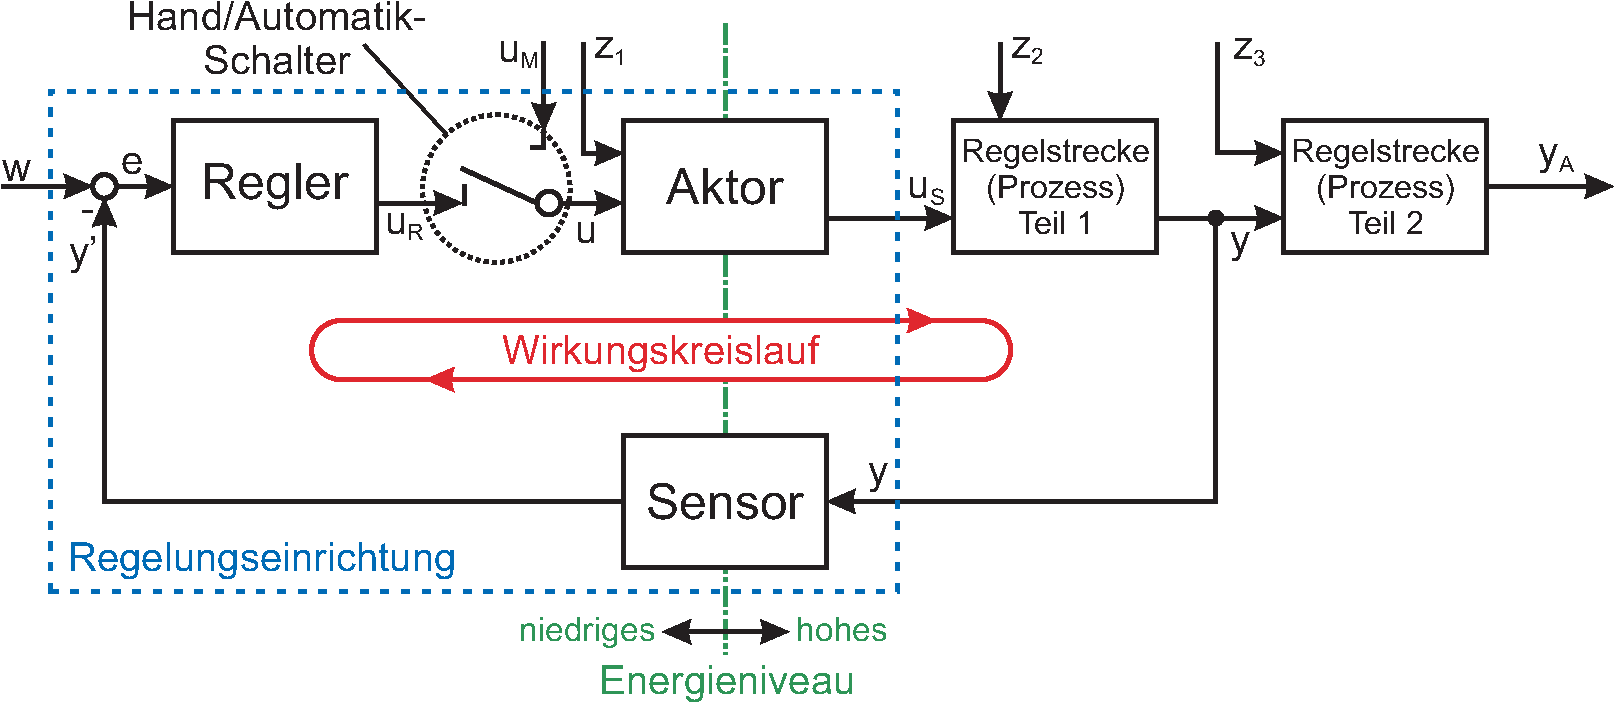
\includegraphics[width=0.95\columnwidth]{Grafiken/Grundelemente_Regelkreis}
\begin{enumerate}[label=$\bullet$]
\item Führungsgröße $\mathbf{w}$:\\
Sollvorgabe für die Aufgabengröße, die es durch den Regler einzuhalten gilt.
\item Regeldifferenz $\mathbf{e}$:\\
Im Idealfall hält der Regler diese Größe stets bei Null; dies ist ein Hauptziel jeder Regelung.
\item Stellgröße $\mathbf{u_S}$:\\
Eingang des zu regelnden Systems, im weiteren auch als Regelstrecke oder Prozess bezeichnet. Stellgrößen werden durch Aktoren erzeugt; sie bewirken auch die Signalwandlung von niedrigem auf hohes Energieniveau innerhalb der Regelschleife.
\item Aktoreingang $\mathbf{u}$:\\
Eingangsgröße des Stellgliedes oder Aktors, die aus der Ausgangsgröße des Reglers $u_R$ (Automatikbetrieb) bzw. eines manuellen Stellelementes $u_M$ (manueller Betrieb) hervorgeht.
\item Aufgabengröße $\mathbf{y_A}$:\\
Die eigentlich zu beeinflussende Größe.
\item Regelgröße $\mathbf{y}$:\\
Die tatsächlich durch einen Sensor erfassbare Größe, die dem Regler zugeführt wird; $y$ kann von $y_A$ mehr oder weniger stark abweichen.
\item Störgrößen $\mathbf{z_i}$:\\
Nicht vorhersehbare und nicht beeinflussbare Größen, die an den verschiedensten Punkten in der Regelschleife angreifen können.
\end{enumerate}

\section{Darstellungen von LTI-SISO-Systemen}

\subsection{Lineare DGL n-ter Ordnung}
\begin{equation*}
a_ny^{(n)}+a_{n-1}y^{(n-1)}+...+a_0y=b_mu^{(m)}+...+b_0u
\end{equation*}

\subsubsection{Transformation aus Zustandsraummodell}
\begin{equation*}
\text{Setze }\underline{x}=\begin{bmatrix}x_1 \\ x_2 \\ \vdots \\ x_n\end{bmatrix}=\begin{bmatrix}y \\ \dot{y} \\ \vdots \\ \overset{(n-1)}{y}\end{bmatrix}
\end{equation*}
Wenn alle $x_n$ durch $\overset{(n-1)}{y}$ ersetzt worden sind, müssen nur noch alle Gleichungen ineinander eingesetzt werden, sodass nur noch eine DGL $n$-ter Ordnung übrig bleibt.

\subsubsection{Transformation aus Übertragungsfunktion}
Die DGL kann mittels inverser Laplace-Transformation der Übertragungsfunktion ermittelt werden.

\subsection{Zustandsraummodell}
\begin{equation*}
\begin{split}
\underline{\dot{x}}&=A\underline{x}+\underline{b}u\\
y&=\underline{c}^T\underline{x}+du
\end{split}
\end{equation*}

\subsubsection{Transformation aus DGL}
Sei $a_n=1$.
\begin{equation*}
\text{Setze }\underline{x}=\begin{bmatrix}x_1 \\ x_2 \\ \vdots \\ x_n\end{bmatrix}=\frac{1}{b_0}\begin{bmatrix}y \\ \dot{y} \\ \vdots \\ \overset{(n-1)}{y}\end{bmatrix}
\end{equation*}
\begin{equation*}
\begin{split}
\Rightarrow \underline{\dot{x}}&=\begin{bmatrix}0 & 1 & 0 & ... & 0 \\ 0 & 0 & 1 & ... & 0 \\
\vdots & \vdots & \vdots & \ddots & \vdots \\ 0 & 0 & 0 & ... & 1 \\ -a_0 & -a_1 & -a_2 & ... & -a_{n-1}\end{bmatrix}\underline{x}+\begin{bmatrix}0 \\ \vdots \\ 0 \\ 1\end{bmatrix}u
\end{split}
\end{equation*}
\begin{equation*}
\begin{split}
\text{Für }&0<m<n\text{ gilt:}\\
y&=[b_0,b_1,...,b_m,0,...,0]\underline{x}\\
\text{Für }&m=n\text{ gilt:}\\
y&=[b_0-a_0b_n,b_1-a_1b_n,...,b_{n-1}-a_{n-1}b_n]\underline{x}+b_nu
\end{split}
\end{equation*}

\subsubsection{Transformation aus Übertragungsfunktion}
Zuerst die Übertragungsfunktion mittels inverser Laplace-Transformation in eine DGL umwandeln und danach wie oben beschrieben vorgehen.

\subsection{Übertragungsfunktion}
\begin{equation*}
G(s)=\frac{Y(s)}{U(s)}
\end{equation*}

\subsubsection{Transformation aus DGL}
Die Übertragungsfunktion kann mittels Laplace-Transformation der DGL ermittelt werden.

\subsubsection{Transformation aus Zustandsmatrix}
\begin{equation*}
G(s)=\underline{c}^T(sI_n-A)^{-1}\underline{b}+d=\frac{det\begin{bmatrix}sI_n-A & -\underline{b} \\ \underline{c}^T & d\end{bmatrix}}{det(sI_n-A)}
\end{equation*}

\subsection{Darstellungsformen von Zustandsraummodellen}

\subsubsection{Kanonische Normalform}
\begin{equation*}
\begin{split}
\underline{\dot{x}}_k&=diag(\lambda_i)\underline{x}_k+\underline{b}_ku\\
y&=\underline{c}_k^T\underline{x}_k+du\\
diag(\lambda_i)&=T^{-1}AT=\begin{bmatrix}\lambda_1 & 0 & ... & 0 \\ 0 & \lambda_2 & ... & 0 \\ \vdots & \vdots & \ddots & \vdots \\ 0 & 0 & ... & \lambda_n\end{bmatrix}
\end{split}
\end{equation*}
mit $T=[\underline{v}_1,\underline{v}_2,...,\underline{v}_n],\;\underline{b}_k=T^{-1}\underline{b},\;\underline{c}_k^T=\underline{c}^TT\;,\underline{x}_k=T^{-1}\underline{x}$\\
$\lambda_i$: Eigenwerte von $A$\\
$\underline{v}_i$: Eigenvektoren von $A$

\subsubsection{Regelungsnormalform}
\begin{equation*}
\begin{split}
\underline{\dot{x}}_R&=A_R\underline{x}_R+\underline{b}_Ru\\
y&=\underline{c}_R^T\underline{x}_R+du\\
A_R&=\begin{bmatrix}0 & 1 & 0 & ... & 0 \\ 0 & 0 & 1 & ... & 0 \\
\vdots & \vdots & \vdots & \ddots & \vdots \\ 0 & 0 & 0 & ... & 1 \\ -a_0 & -a_1 & -a_2 & ... & -a_{n-1}\end{bmatrix};\;\;\;\underline{b}_R=\begin{bmatrix}0 \\ 0 \\ \vdots \\ 1\end{bmatrix}\\
\underline{c}_R^T&=[b_0-b_na_0,b_1-b_na_1,...,b_{n-1}-b_na_{n-1}]\\
d&=b_n
\end{split}
\end{equation*}\\\\
\textbf{Transformation eines beliebigen Systems in Regelungsnormalform:}\\
\begin{enumerate}
\item Steuerbarkeitsmatrix aufstellen:
\begin{equation*}
Q_c=[\underline{b},A\underline{b},A^2\underline{b},...,A^{n-1}\underline{b}]
\end{equation*}
\item Letzte Zeile von $Q_c^{-1}$:
\begin{equation*}
\underline{q}_c^T=[0,0,...,0,1]Q_c^{-1}
\end{equation*}
\item Transformationsmatrix:
\begin{equation*}
T_R=\begin{bmatrix}\underline{q}_c^T \\ \underline{q}_c^TA \\ \underline{q}_c^TA^2 \\ \vdots \\ \underline{q}_c^TA^{n-1}\end{bmatrix}^{-1}
\end{equation*}
\end{enumerate}

\subsubsection{Beobachtungsnormalform}
\begin{equation*}
\begin{split}
\underline{\dot{x}}_B&=\underline{A}_B\underline{x}_B+\underline{b}_Bu\\
y&=\underline{c}_B^T\underline{x}_B+du\\
A_B&=\begin{bmatrix}0 & 0 & ... & 0 & -a_0 \\ 1 & 0 & ... & 0 & -a_1 \\ 0 & 1 & ... & 0 & -a_2 \\ \vdots & \vdots & \ddots & \vdots & \vdots \\ 0 & 0 & ... & 1 & -a_{n-1}\end{bmatrix};\;\;\;\;\underline{b}_B=\begin{bmatrix}b_0-b_na_0 \\ b_1-b_na_1 \\ \vdots \\ b_{n-1}-b_na_{n-1}\end{bmatrix}\\
\underline{c}_B^T&=[0,0,...,1]\\
d&=b
\end{split}
\end{equation*}\\\\
\textbf{Transformation eines beliebigen Systems in Beobachtungsnormalform:}\\
\begin{enumerate}
\item Beobachtbarkeitsmatrix aufstellen:
\begin{equation*}
Q_O=\begin{bmatrix}\underline{c}^T \\ \underline{c}^TA \\ \underline{c}^TA^2 \\ \vdots \\ \underline{c}^TA^{n-1}\end{bmatrix}
\end{equation*}
\item Letzte Spalte von $Q_O^{-1}$:
\begin{equation*}
\underline{q}_O=Q_O^{-1}[0,...,0,1]^T
\end{equation*}
\item Transformationsmatrix:
\begin{equation*}
T_B=[\underline{q}_O,A\underline{q}_O,...,A^{n-1}\underline{q}_O]
\end{equation*}
\end{enumerate}
\textbf{Zusammenhang zwischen Regelungs- und Beobachtungsnormalform:}
\begin{equation*}
A_R=A_B^T,\;\;\;\;\;\underline{b}_R=\underline{c}_B,\;\;\;\;\;\underline{c}_R=\underline{b}_B
\end{equation*}

\section{Blockschaltbilder}

\subsection{Kreisstruktur}
\begin{minipage}[b]{0.45\columnwidth}
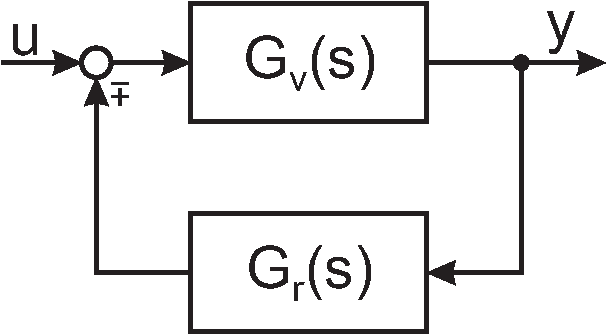
\includegraphics[width=0.9\textwidth]{Grafiken/Kreisstruktur}
\end{minipage}
\hfill
\begin{minipage}[b]{0.55\columnwidth}
$G(s)=\frac{G_v(s)}{1\pm G_v(s)G_r(s)}$\\\\
\end{minipage}

\section{Zeitverhalten linearer dynamischer Systeme}

\subsection{Lösung eines linearen DGL-Systems}
Sei
\begin{equation*}
\begin{split}
\underline{\dot{x}}&=A\underline{x}+B\underline{u}\\
\underline{y}&=C\underline{x}+D\underline{u}
\end{split}
\end{equation*}
dann lautet die Lösung:
\begin{equation*}
x(t)=\underbrace{\Phi(t-t_0)x_0}_{\text{Eigenbewegung}}+\underbrace{\int\limits_{t_0}^{t}\Phi(t-\tau)B\underline{u}(\tau)d\tau}_{\text{Erzwungene Bewegung}};\;\;\;t\geq t_0
\end{equation*}
mit $\Phi(t)=e^{At}$.

\subsection{Anfangs- und Endwertsatz der Laplace-Transformation}

\subsubsection{Anfangswertsatz}
\begin{equation*}
y(t\rightarrow 0^+)=\lim\limits_{s\rightarrow\infty}[sG(s)U(s)]
\end{equation*}

\subsubsection{Endwertsatz}
\begin{equation*}
y(t\rightarrow\infty)=\lim\limits_{s\rightarrow 0}[sG(s)U(s)]
\end{equation*}
Voraussetzung für die Anwendbarkeit der Grenzwertsätze ist, dass die Grenzwerte auf beiden Seiten existieren.

\subsection{Kennwerte der Übertragungfunktion}
\begin{center}
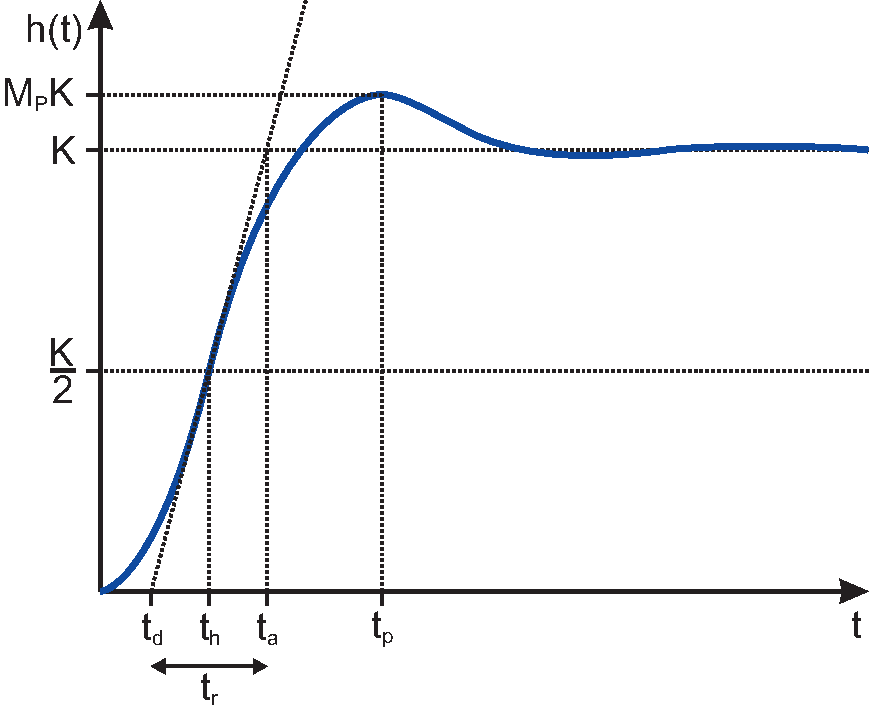
\includegraphics[width=0.95\columnwidth]{Grafiken/Kennwerte_Uebertragungsfunktion}
\end{center}
\begin{tabular}{ll}
$K$: & Stationärer Endwert\\
$t_h$: & Zeitpunkt des halben Endwertes\\
$t_r$: & Anstiegszeit\\
$t_d$: & Verzugszeit\\
$t_a$: & Anregelzeit\\
$T_{ein}$: & Die kleinste Zeit, nach der $h(t)$ von Endwert $K$\\
& um maximal 5\% abweicht.\\
$t_p$: & Zeitpunkt des maximalen Überschwingens
\end{tabular}




\section{Systemdynamische Bausteine}

\subsection{Totzeitsysteme}
\begin{equation*}
y(t)=Ku(t-T_t)\laplace G(s)=Ke^{-sT_t}
\end{equation*}

\subsubsection{Rationale Approximationen}
\begin{enumerate}[label=$\bullet$]
\item Reihenentwicklung ($PT_n$-System)
\begin{equation*}
\begin{split}
e^{-sT_t}&\approx\frac{1}{\left(1+\frac{sT_t}{n}\right)^n},\;\;\;n\geq 1\\
\text{bzw. }e^{-sT_t}&\approx\frac{1}{1+sT_t},\;\;\;n=1
\end{split}
\end{equation*}
\item Padé-Approximation
\begin{equation*}
e^{-sT_t}\approx\frac{1-s\frac{T_t}{2}}{1+s\frac{T_t}{2}}
\end{equation*}
\end{enumerate}

\subsection{Minimalphasensysteme und Allpässe}

\subsubsection{Minimalphasensysteme (MP)}
MP-Systeme haben keine Nullstellen oder/und Pole in der rechten Halbebene der Pol-/Nullstellenkarte, d.h.
\begin{equation*}
Re\{q_{\mu}\}\leq 0,\;\;\;\;Re\{p_{\nu}\}\leq 0\;\;\;\;\forall\mu,\nu
\end{equation*}

\subsubsection{Nichtminimalphasensysteme (NMP)}
NMP-Systeme sind Systeme, die mindestens eine Pol- oder Nullstelle in der rechten Halbebene haben und/oder totzeitbehaftet sind.\\
Jedes NMP-System kann in kann in eine Serienschaltung aus MP- und AP-System aufgespalten werden.\\\\
Sowohl bei NMP- als auch bei AP-Systemen stellt sich anfänglich eine Umkehr des Wirkungssinns ein.

\subsubsection{Allpasssysteme (AP)}
AP-Systeme sind spezielle NMP-Systeme, deren Pol-/Nullstellenverteilung symmetrisch zur Imaginärachse der $s$-Ebene ist. AP-Systeme haben eine frequenzunabhängigen, konstanten Amplitudenverlauf $|G(j\omega)|$.

\section{Stabilität}

\subsection{Zustandsstabilität}
Ein System ist zustandsstabil, wenn gilt:
\begin{equation*}
Re\{\lambda_i(A)\}<0\;\;\forall i
\end{equation*}

\subsection{Routh-Hurwitz-Kriterium}
Gegeben sei das charakteristische Polynom (Nennerpolynom von $G(s)$):
\begin{equation*}
N(s)=b_ns^n+b_{n-1}s^{n-1}+...+b_0
\end{equation*}
Ein System ist stabil, wenn gilt:
\begin{equation*}
b_n>0\;\;\forall n\;\;\text{\textbf{und} alle }n\;\text{Hurwitzdeterminanten}>0
\end{equation*}

\subsubsection{Spezialfälle}
\begin{equation*}
\begin{split}
n=1:&\;\;\;b_1>0,\;b_0>0\\
n=2:&\;\;\;b_2>0,\;b_1>0,\;b_0>0\\
n=3:&\;\;\;b_3>0,\;b_2>0,\;(b_1>0),\;b_0>0,\;b_2b_1-b_0b_3>0\\
n=4:&\;\;\;b_4>0,\;b_3>0,\;(b_2>0),\;b_1>0,\;b_0>0,\\
&\;\;\;b_3b_2b_1-b_0b_3^2-b_1^2b_4>0
\end{split}
\end{equation*}

\subsection{Direkte Methode von Lyapunov}
Nach Lyapunov ist der GGP $\underline{x}^*$ einer DGL $\underline{\dot{x}}=f(\underline{x})$ asymptotisch stabil, wenn eine Lyapunov-Funktion $V(\underline{x})$ gefunden werden kann mit den Eigenschaften:
\begin{enumerate}
\item $V(\underline{x}^*)=0$
\item $V(\underline{x})>0\text{ für alle }\underline{x}$
\item $\frac{d}{dt}V(\underline{x})<0\text{ für alle Lösungen der DGL}$
\end{enumerate}

\subsubsection{Spezialfall: lineare Systeme mit regulärer Systemmatrix $A$}
Falls $\underline{\dot{x}}=A\underline{x}$, lautet der Ansatz:
\begin{equation*}
V(\underline{x})=\underline{x}^TP\underline{x}
\end{equation*}
Seien $P$ und $Q$ symmetrische, positiv definite Matrizen und gelte:
\begin{equation*}
A^TP+PA=-Q
\end{equation*}
Vorgehensweise, um asymptotische Stabilität nachzuweisen:
\begin{enumerate}
\item Wähle $Q$ als symmetrische, positiv definite Matrix (z.B. $Q=I_n$)
\item Einsetzen von allgemeinem symmetrischen Ansatz für $P$:
\begin{equation*}
P=\begin{bmatrix}p_1 & p_2 & ... \\ p_2 & p_3 & \vdots \\ \vdots & ... & \ddots\end{bmatrix}
\end{equation*}
\item
\begin{enumerate}[label=$\bullet$]
\item Falls $P$ nicht positiv definit\\
$\Rightarrow$ System nicht asymptotisch stabil
\item Falls $P$ positiv definit\\
$\Rightarrow$ System asymptotisch stabil
\end{enumerate}
\end{enumerate}
Eine symmetrische Matrix ist positiv definit, falls gilt:
\begin{equation*}
\lambda_i>0\;\;\forall i
\end{equation*}

\subsection{Zustandssteuerbarkeit und Zustandsbeobachtbarkeit}

\subsubsection{Steuerbarkeitskriterium}
Ein System $\underline{\dot{x}}=A\underline{x}+B\underline{u}$ ist nur dann vollständig zustandssteuerbar, wenn gilt:
\begin{equation*}
\begin{split}
Rang(Q_c)&=n\\
\text{bzw. }det(Q_c)&\neq 0\;\;\;\text{für SISO/SIMO-Systeme}
\end{split}
\end{equation*}
mit der $n\times (n\cdot r)$-Steuerbarkeitsmatrix
\begin{equation*}
Q_c=[B,AB,...,A^{n-1}B]
\end{equation*}
Der Rang der Matrix $Q_c$ entspricht der Anzahl der steuerbaren Zustände.

\subsubsection{Beobachtbarkeitskriterium}
Ein System $\underline{\dot{x}}=A\underline{x},\;\underline{y}=C\underline{x}$ ist nur dann vollständig zustandsbeobachtbar, wenn gilt:
\begin{equation*}
\begin{split}
Rang(Q_O)&=n\\
\text{bzw. }det(Q_O)&\neq 0\;\;\;\text{für SI/MISO-Systeme}
\end{split}
\end{equation*}
mit der $n\times (n\cdot q)$-Beobachtbarkeitsmatrix
\begin{equation*}
Q_O=[C^T,A^TC^T,...,(A^T)^{n-1}C^T]
\end{equation*}
Der Rang der Matrix $Q_O$ entspricht der Anzahl der beobachtbaren Zustände.

\subsubsection{Einfluss von Steuerbarkeit und Beobachtbarkeit auf das E/A-Verhalten}
Jedes SISO-LTI-System kann durch geeignete Transformation in 4 Subsysteme zerlegt werden:
\begin{center}
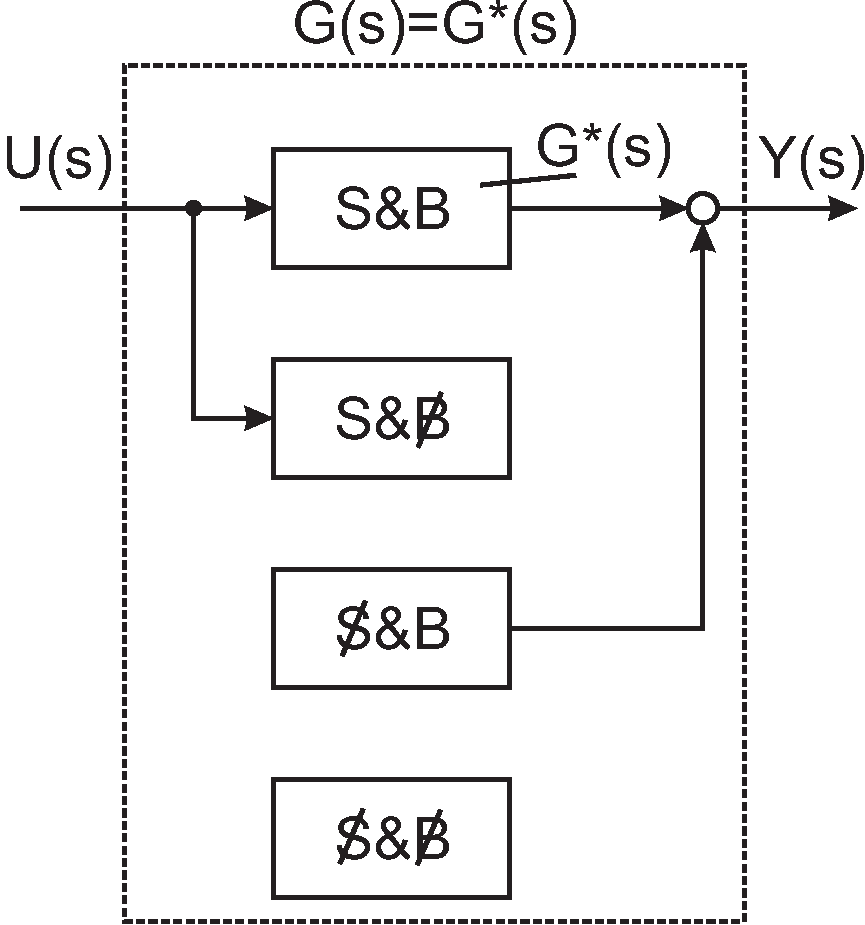
\includegraphics[width=0.6\columnwidth]{Grafiken/Aufteilung_SISO}
\end{center}
Ein SISO-LTI-System hat nur dann eine nicht-reduzierbare E/A-Übertragungsfunktion $G(s)$, wenn das System vollständig steuerbar und beobachtbar ist.\\
Umgekehrt ist alleine aufgrund einer gegebenen - möglicherweise reduzierten - E/A-Übertragungsfunktion kein eindeutiger Schluss auf die Zustandsbeschreibung und die zugehörigen Eigenwerte möglich.

\subsection{BIBO(E/A)-Stabilität (äußere Stabilität)}
Bei E/A-stabilen Systemen gilt für die Pole der Übertragungsfunktion:
\begin{equation*}
Re\{p_i\}<0;\;\;\;\;i=1,2,...,n
\end{equation*}

\subsubsection{E/A-Stabilitätsbedingungen}
\begin{enumerate}[label= $\bullet$]
\item Ist ein System vollständig steuerbar und beobachtbar und $Re\{\lambda_i(A)\}<0\;\;\forall i$, dann gilt:
\begin{equation*}
\text{asymptotisch stabil }\Leftrightarrow\text{ E/A-stabil}
\end{equation*}
\item Ist ein System nicht vollständig steuerbar und/oder nicht vollständig beobachtbar, aber es gilt für alle steuerbaren und beobachtbaren Eigenwerte $Re\{\lambda_i(A)\}<0$, dann folgt:
\begin{equation*}
\text{asymptotisch stabil }\Rightarrow\text{ E/A-stabil}
\end{equation*}
\end{enumerate}

\subsection{Stabilitätsgrad}
\begin{center}
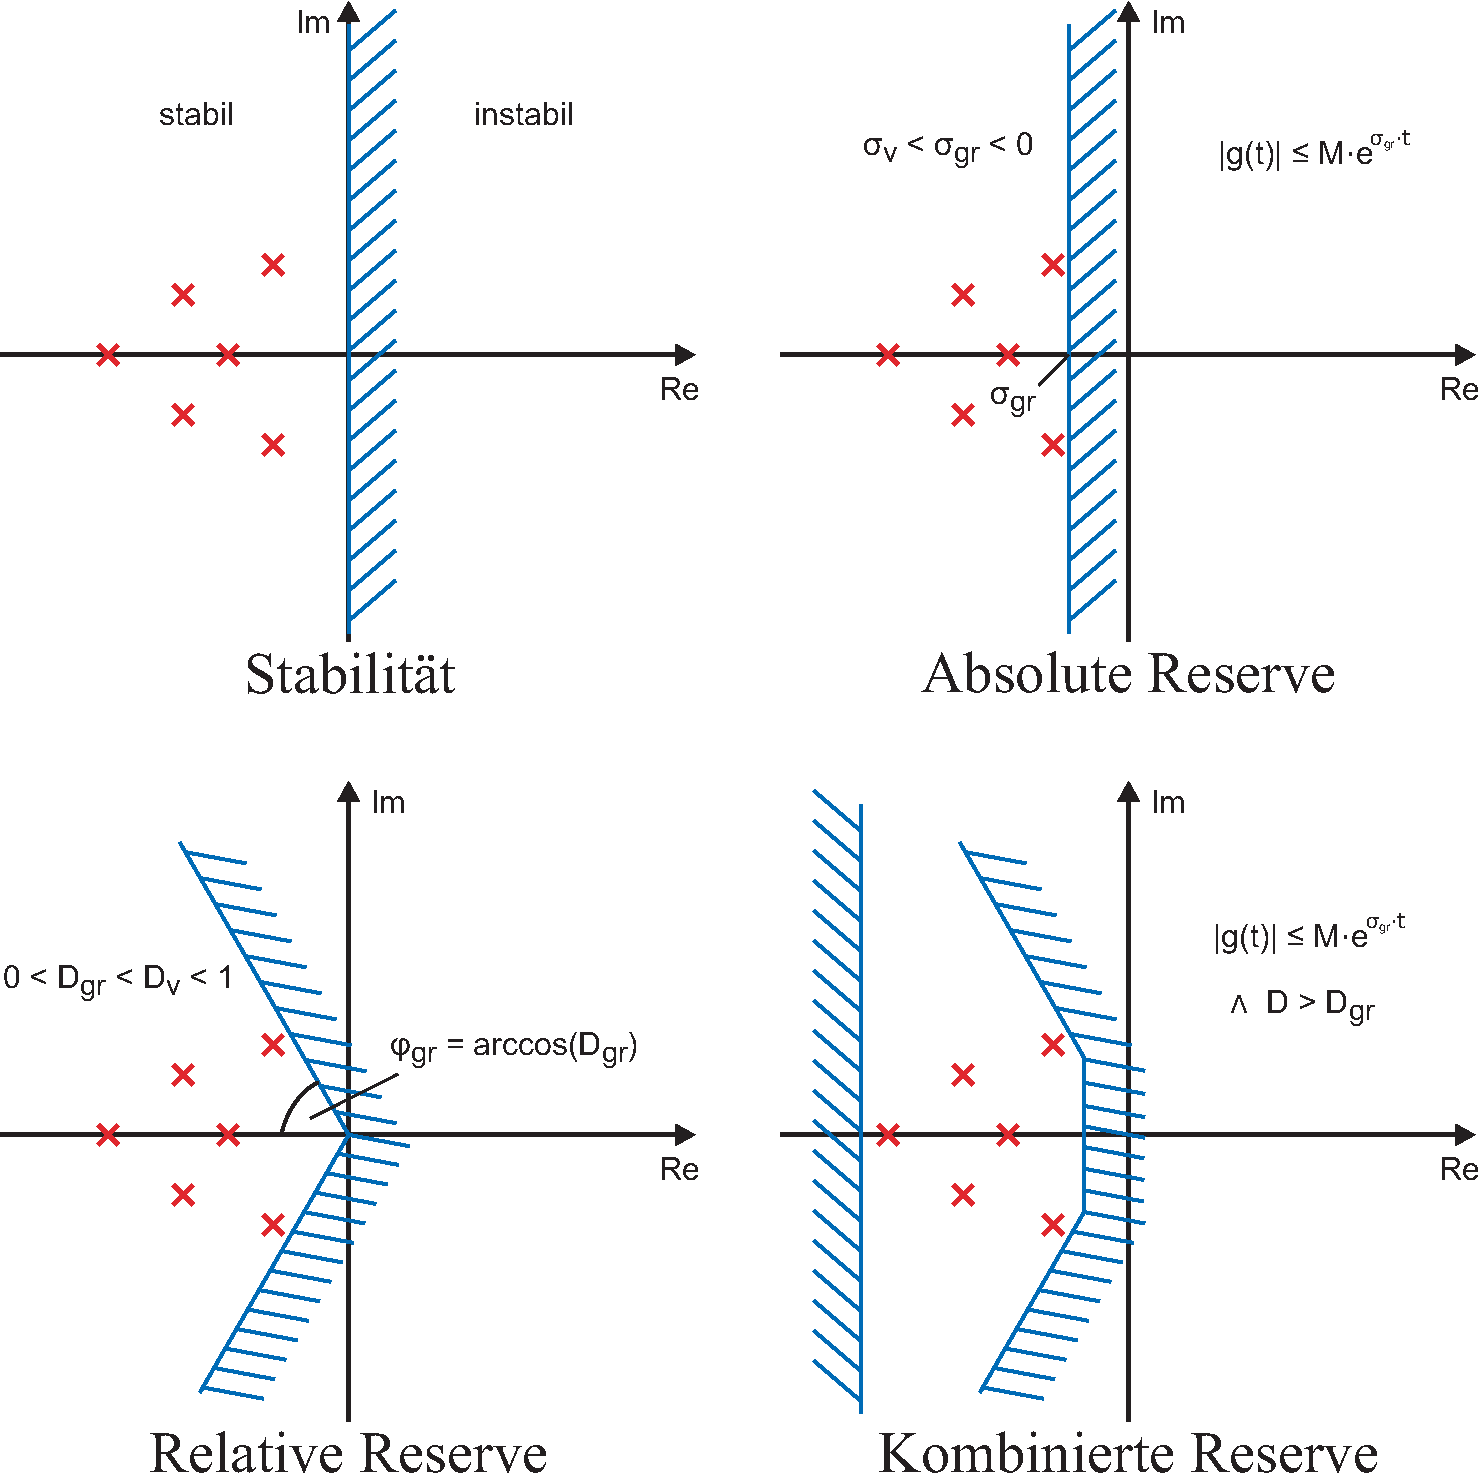
\includegraphics[width=0.95\columnwidth]{Grafiken/Stabilitaetsreserven}
\end{center}

\subsection{Dominierendes Systemverhalten und Ordnungsreduktion}
Diejenigen Pole, die näher an der Imaginärachse liegen, dominieren das Systemverhalten.\\
Falls der Faktor mindestens 10 beträgt, kann der nicht dominierende Teil vernachlässigt werden.\\
Grenz- oder instabile Pole sind immer dominant und dürfen daher nie gestrichen werden!\\\\
\textbf{Achtung:}\\
Für die Reduktion muss $G(s)$ in Zeitkonstantenform umgeschrieben werden!

\subsubsection{Beispiel}
\begin{equation*}
G(s)=\frac{2}{(1+s)(1+0,1s)}=\underbrace{\frac{2}{1+s}}_{\text{dom.}}\cdot\underbrace{\frac{1}{1+0,1s}}_{\text{nicht dom.}}\approx\frac{2}{1+s}
\end{equation*}

\section{Grundlagen der Regelung und Standardregler}

\subsection{Standardstrecken}

\subsubsection{Strecke vom globalen P-Typ}
\begin{equation*}
G(s)=K_s\cdot\frac{1+...s+...s^2+...}{1+...s+...s^2+...}
\end{equation*}

\subsubsection{Strecke vom globalen I-Typ}
\begin{equation*}
G(s)=\frac{K_s}{s}\cdot\frac{1+...s+...s^2+...}{1+...s+...s^2+...}
\end{equation*}

\subsection{Standardregler}

\subsubsection{PID-Regler}
Da der PID-Regler nicht kausal und somit nicht realisierbar ist, wird in der Realität ein verzögerter PID-Regler verwendet:
\begin{equation*}
G_R(s)=K_P+\frac{K_I}{s}+\frac{K_Ds}{1+Ts}
\end{equation*}

\subsubsection{Vorhalt/Nacheil-Regler}
\begin{equation*}
G_R(s)=K_P\cdot\frac{1+T_vs}{1+Ts};\;\;\;\;T_v,T>0
\end{equation*}
$T_v>T$: Vorhalt-Regler ($PDT_1$)\\
$T_v<T$: Nacheil-Regler ($PI$-ähnlich)

\subsection{Stationäres Regelkreisverhalten}
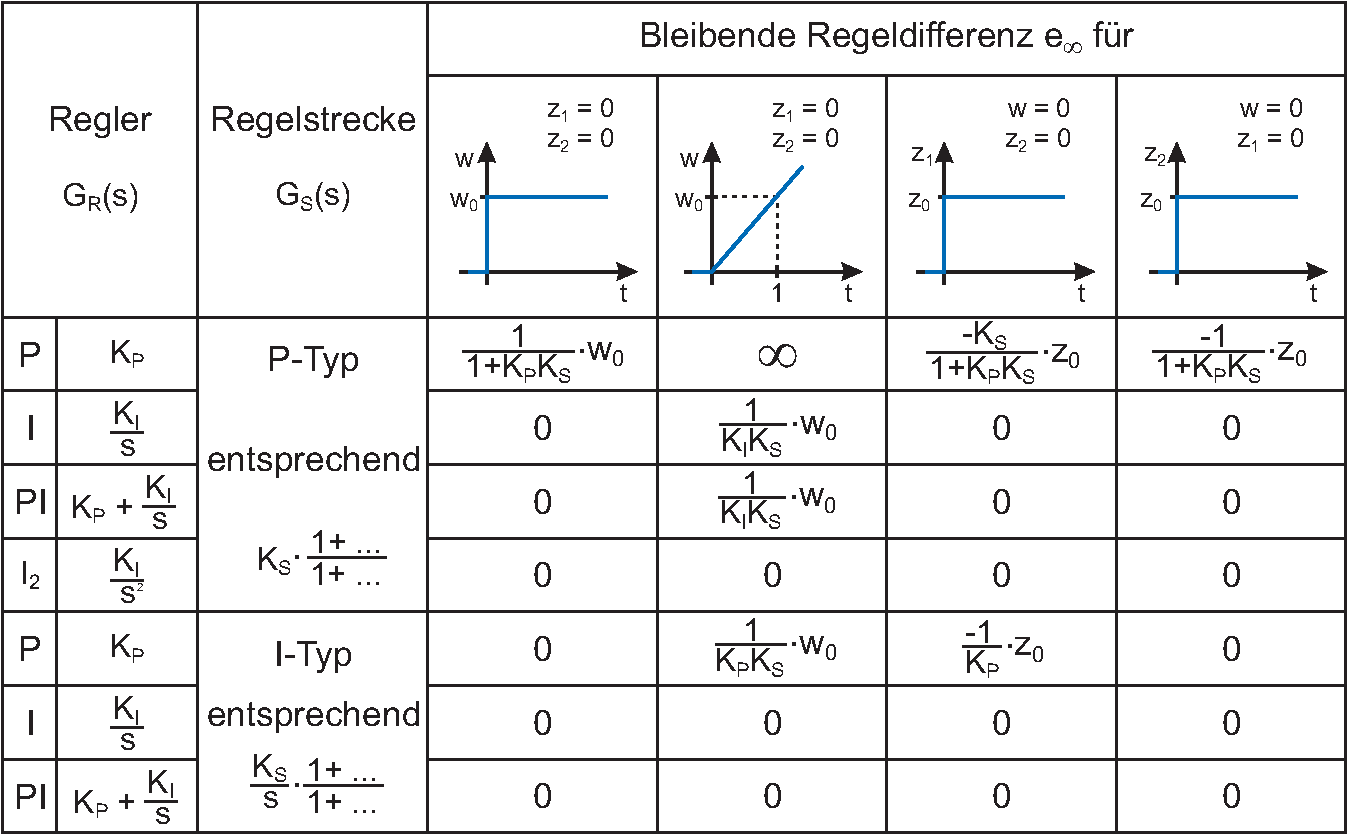
\includegraphics[width=0.98\columnwidth]{Grafiken/Stat_Regelkreisverhalten}

\section{Stabilitätsanalyse im Frequenzbereich}

\subsection{Nyquist-Ortskurve}

\subsubsection{Schwingbedingung in Regelkreisen}
Für die Übertragungsfunktion des aufgeschnittenen Regelkreises muss gelten:
\begin{equation*}
G_0(j\omega)\sollsein -1
\end{equation*}

\subsubsection{Nyquist-Kriterium}
Ein geschlossener linearer Regelkreis ist dann stabil, wenn die Ortskurve des aufgeschnittenen Regelkreises $G_0(j\omega)$
\begin{enumerate}
\item nicht durch den kritischen Punkt $P_{krit}=-1+0j$ verläuft und
\item der von $P_{krit}$ zum laufenden Ortskurvenpunkt $G_0(j\omega)$ weisende Vektor für wachsendes $\omega$ von $+0$ bis $+\infty$ eine globale Phasenwinkeländerung $W$ von
\begin{equation*}
W_{soll}=\overset{\omega=+\infty}{\underset{\omega=+0}{\Delta}}\Phi=n_r\cdot\pi+n_a\cdot\frac{\pi}{2}
\end{equation*}
erfährt.
\end{enumerate}
\begin{tabular}{ll}
$n_r$: & Anzahl der Pole von $G_0(s)$ rechts von der\\
& Imaginärachse\\
$n_a$: & Anzahl der Pole von $G_0(s)$ auf der Imaginärachse
\end{tabular}
\begin{center}
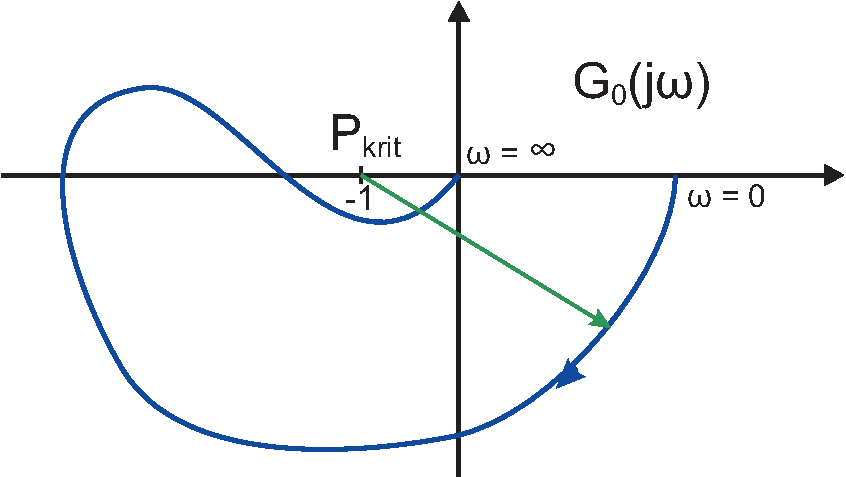
\includegraphics[width=0.8\columnwidth]{Grafiken/Nyquist_Kriterium}
\end{center}

\subsubsection{Linke-Hand-Regel}
Nur anwendbar, wenn $n_r=0$ und $n_a\leq 1$.\\\\
Die Linke-Hand-Regel lautet:\\
Der geschlossene Regelkreis ist stabil, wenn beim Entlangwandern auf der $G_0(j\omega)$-Ortskurve von $\omega=0$ nach $\omega=\infty$ der kritische Punkt $P_{krit}$ beim Passieren des diesem am nächsten liegenden Ortskurvenabschnittes stets auf der linken Seite liegt.

\subsection{Bodediagramme}

\subsubsection{$P$-, $I$-, $D$-Bausteine}
\begin{equation*}
G_P(j\omega)=K_1,\;\;\;\;G_I(j\omega)=\frac{K_2}{j\omega},\;\;\;\;G_D(\jmath\omega)=K_3j\omega
\end{equation*}
\begin{center}
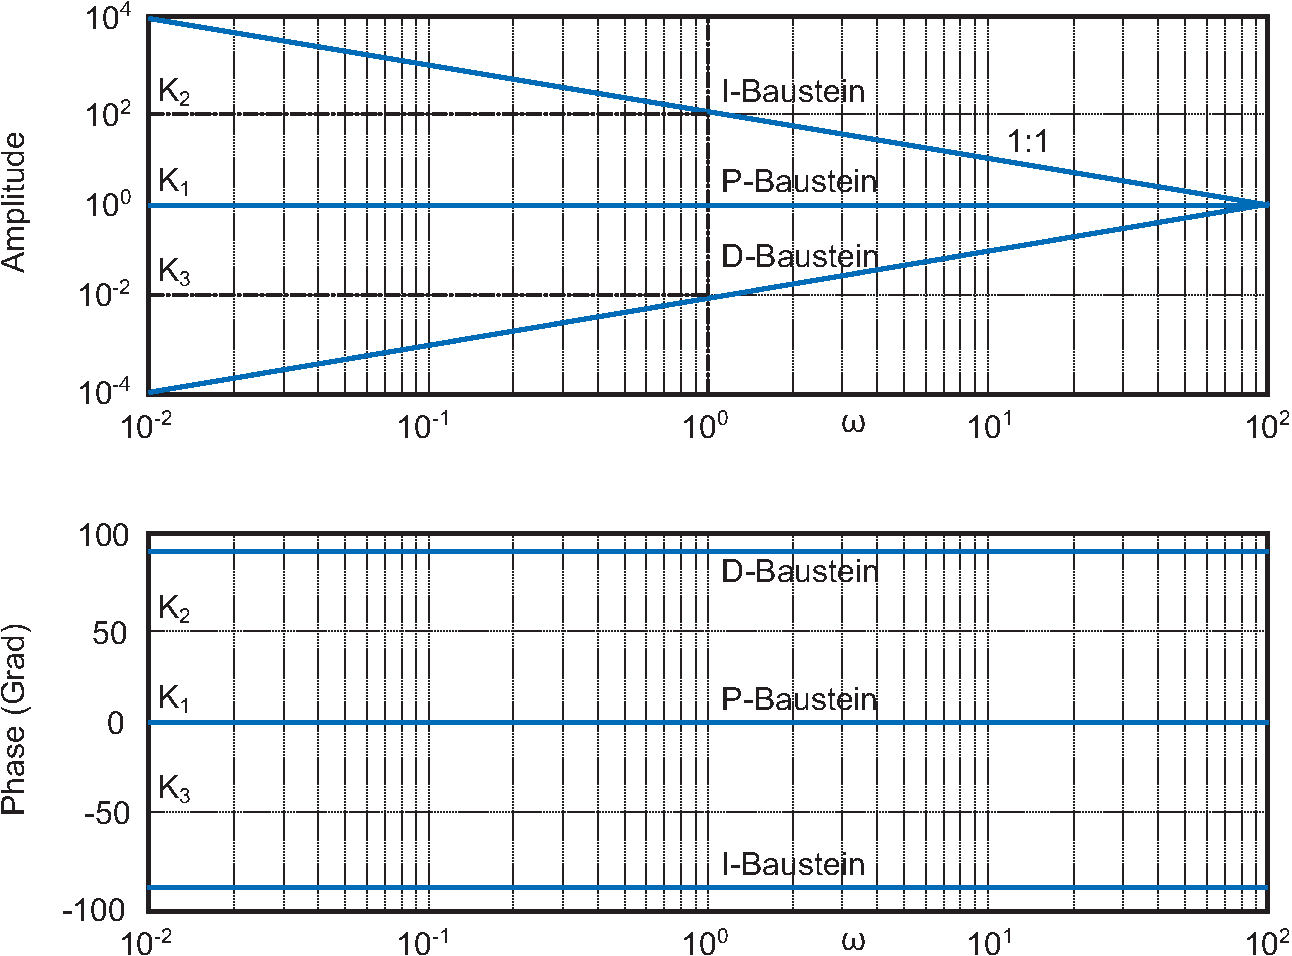
\includegraphics[width=0.95\columnwidth]{Grafiken/Bodediagramme_P_I_D}
\end{center}

\subsubsection{$PT_1$-Bautstein}
\begin{equation*}
G_{PT_1}(j\omega)=\frac{K}{1+j\omega T},\;\;\;\;K,T>0
\end{equation*}
Die Eckfrequenz bzw. Bandbreite $\omega_E$ bezeichnet die Stelle, an der $G(s)$ auf $\frac{G(s)}{\sqrt{2}}$ gefallen ist.
Es gilt außerdem:
\begin{equation*}
\omega_E=\frac{1}{T}
\end{equation*}
\begin{center}
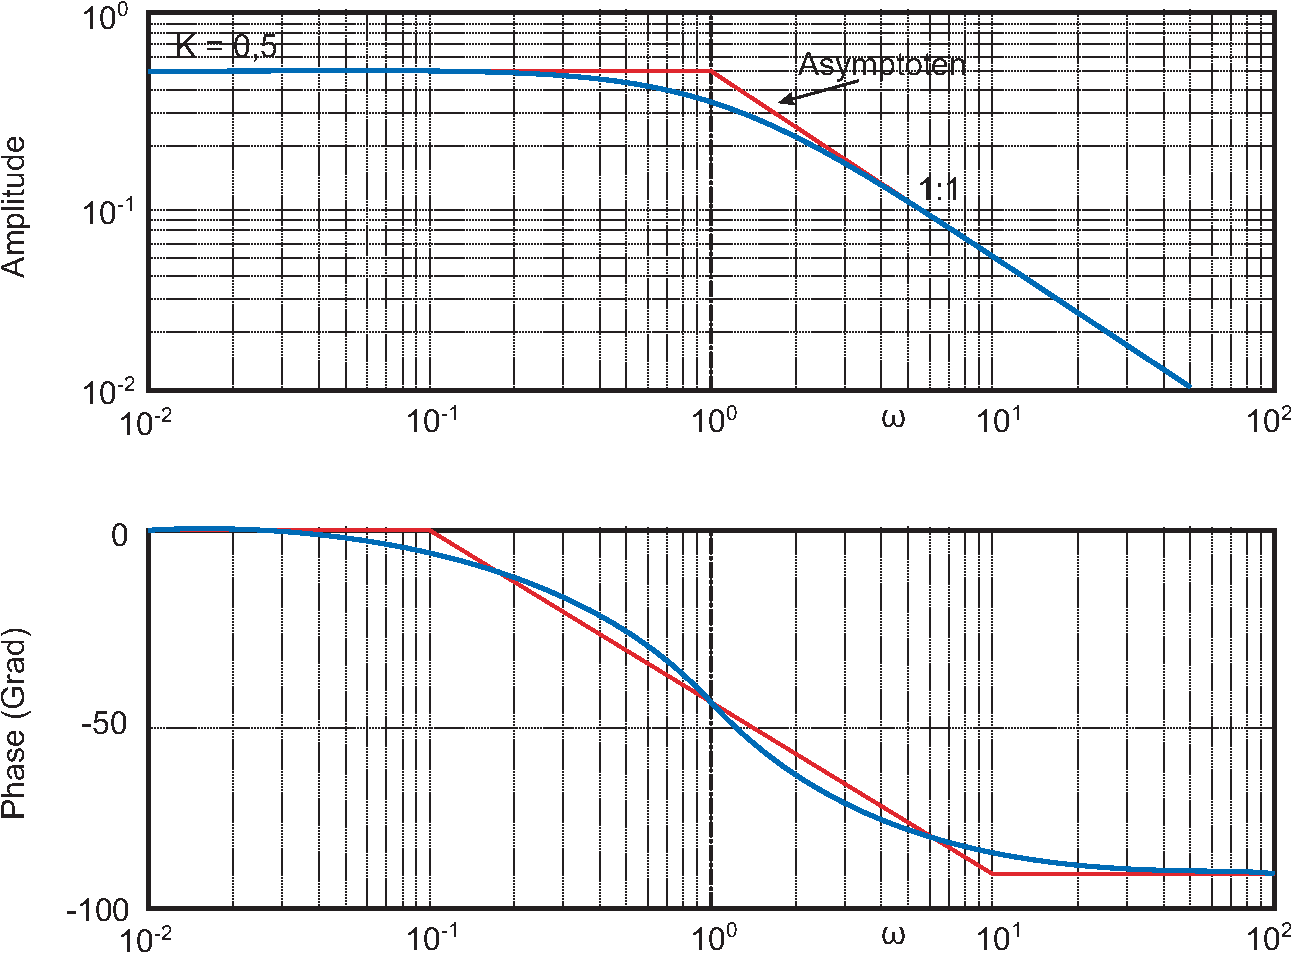
\includegraphics[width=0.95\columnwidth]{Grafiken/Bodediagramm_PT1}
\end{center}

\subsubsection{$PD$-Baustein}
\begin{equation*}
G_{PD}(j\omega)=K\left(1+j\frac{\omega}{\omega_D}\right),\;\;\;\;\omega_D=\frac{1}{T_v},\;\;\;\;K,T_v>0
\end{equation*}
\begin{center}
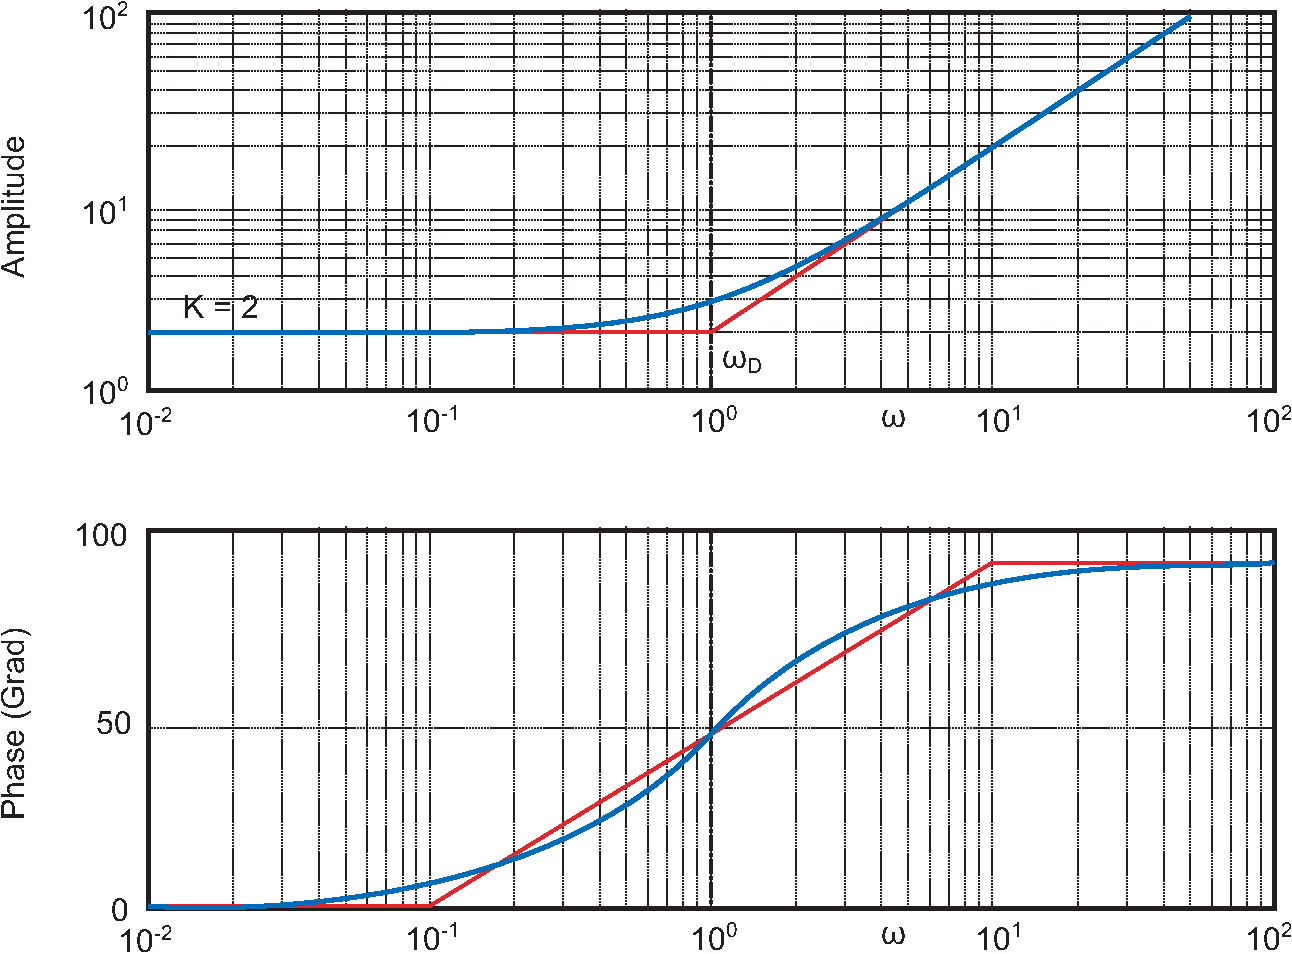
\includegraphics[width=0.95\columnwidth]{Grafiken/Bodediagramm_PD}
\end{center}

\subsubsection{$PT_2$-Baustein}
\begin{equation*}
G_{PT_2}=\frac{K}{1+2D\frac{j\omega}{\omega_0}+\left(\frac{j\omega}{\omega_0}\right)^2},\;\;\;\;0<D<1,K>0
\end{equation*}
Für $0<D<\frac{1}{\sqrt{2}}$ besteht die Fähigkeit zur Resonanz:
\begin{equation*}
\begin{split}
\omega_r&=\omega_0\sqrt{1-2D^2}\\
\text{mit }A_{\text{max}}&=A(\omega_r)=\frac{K}{2D\sqrt{1-D^2}}
\end{split}
\end{equation*}
\begin{center}
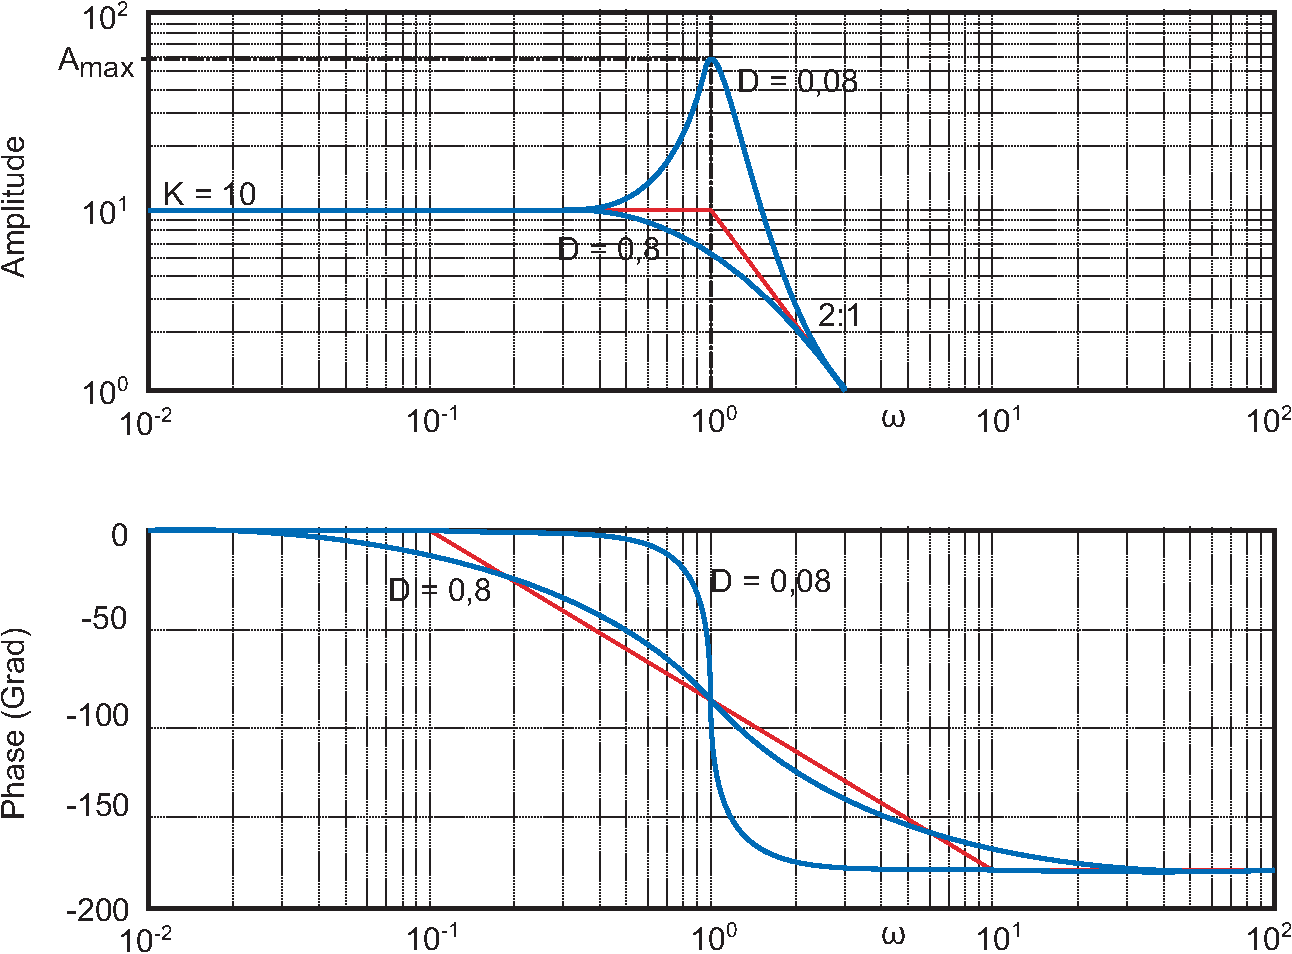
\includegraphics[width=0.95\columnwidth]{Grafiken/Bodediagramm_PT2}
\end{center}

\subsubsection{$T_t$-Baustein}
\begin{equation*}
G_{T_t}(j\omega)=Ke^{-j\omega T_t},\;\;\;\;T_t>0,K>0
\end{equation*}
\begin{center}
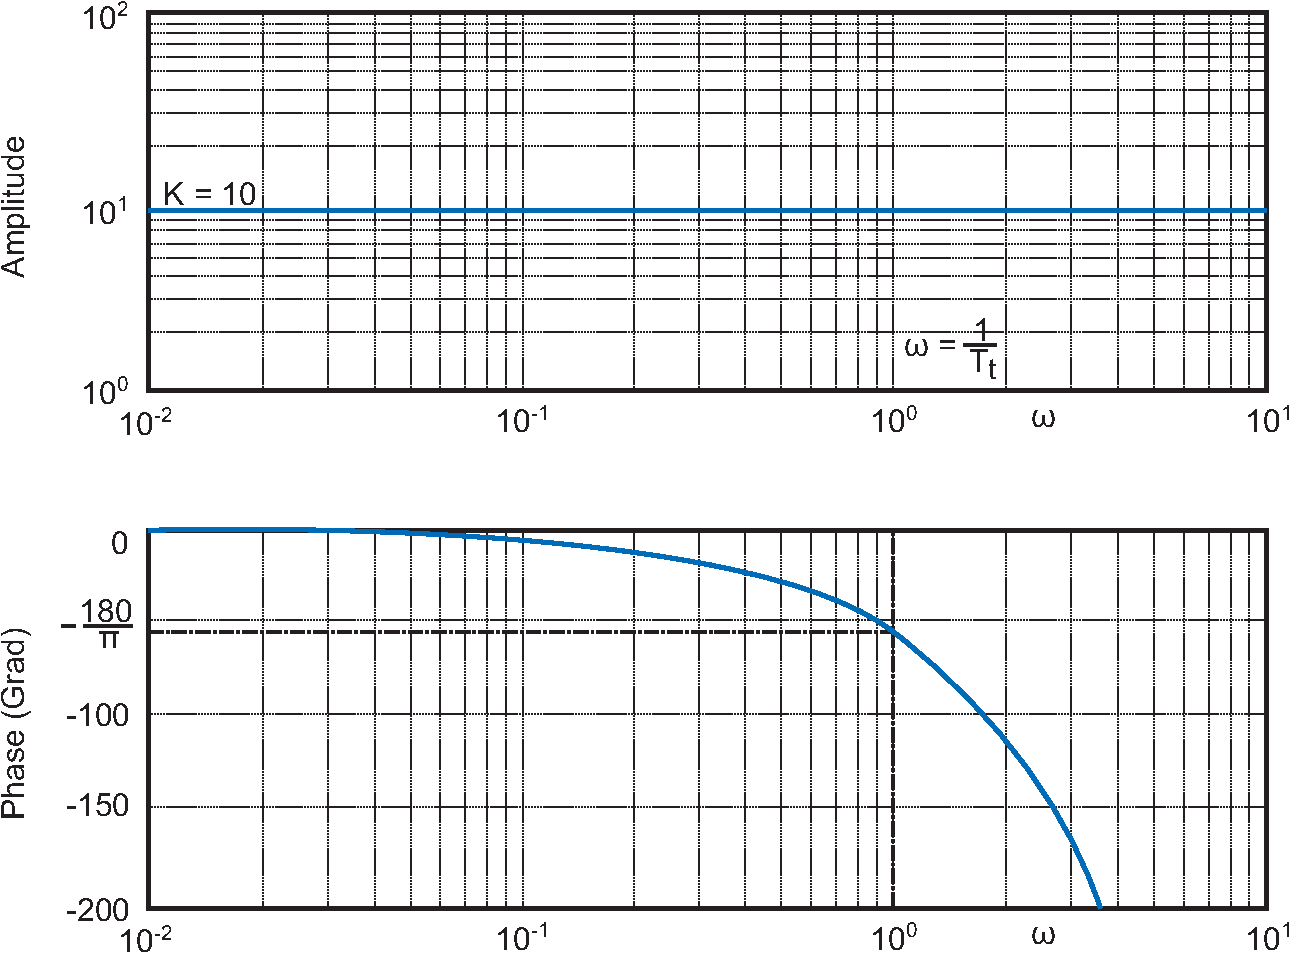
\includegraphics[width=0.95\columnwidth]{Grafiken/Bodediagramm_Tt}
\end{center}

\subsection{Kenngrößen der Frequenzgangfunktion $G_0(j\omega)$}
\begin{enumerate}[label=$\bullet$]
\item Amplituden-Durchtrittsfrequenz $\omega_{D1}$ definiert durch $A(\omega_{D1})=1$
\item Phasen-Durchtrittsfrequenz $\omega_{D2}$ definiert durch $\varphi(\omega_{D2})=-\pi$
\item Phasenrand / Phasenreserve $\Psi_R$ definiert als\\
$\Psi_R=\varphi(\omega_{D1})+\pi$
\item Amplitudenrand / Amplitudenreserve $A_R$ definiert als $\frac{1}{A_R}=A(\omega_{D2})$
\end{enumerate}
\begin{center}
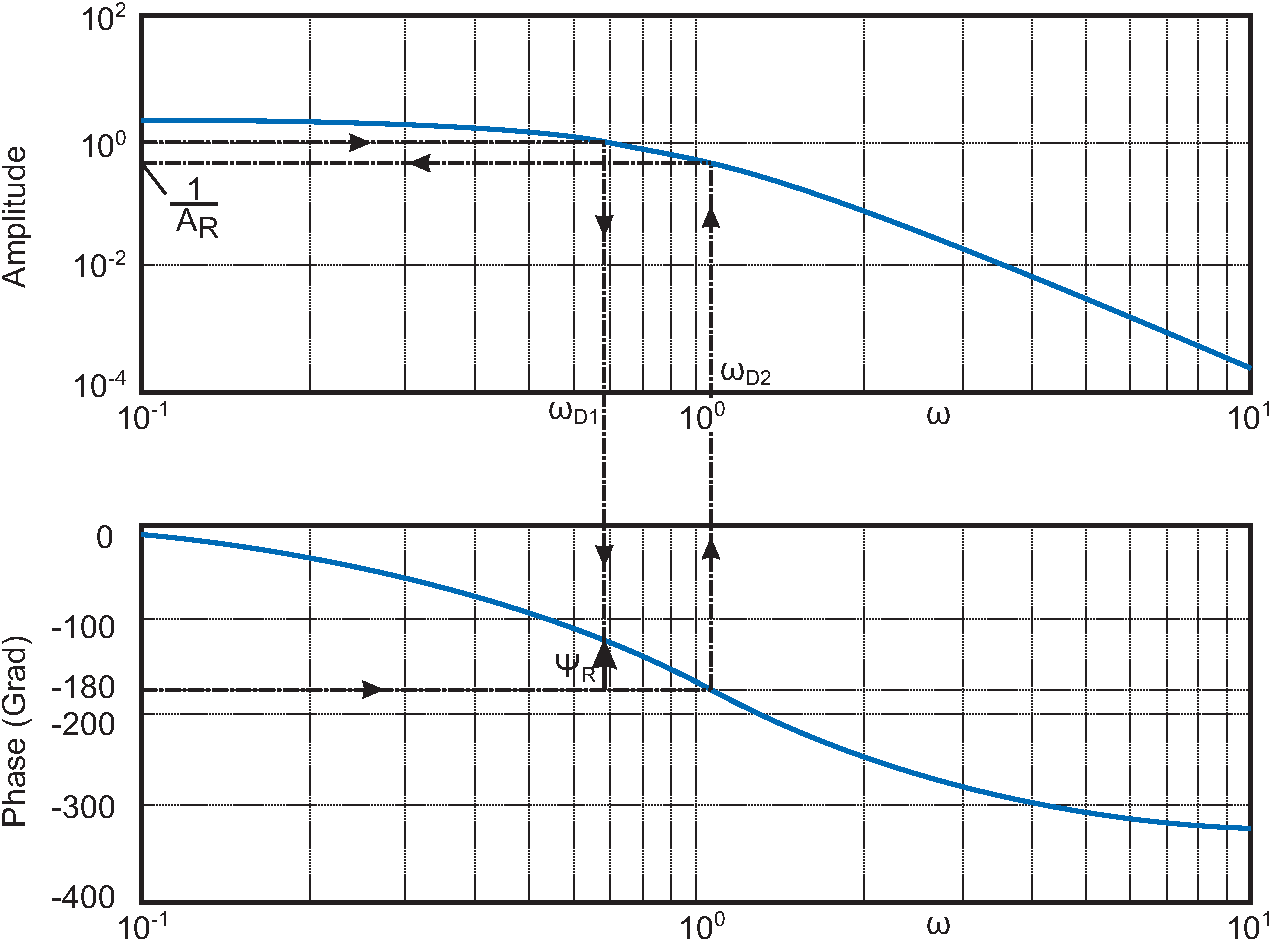
\includegraphics[width=0.95\columnwidth]{Grafiken/Kenngroessen_Bodediagramm}
\end{center}
\begin{center}
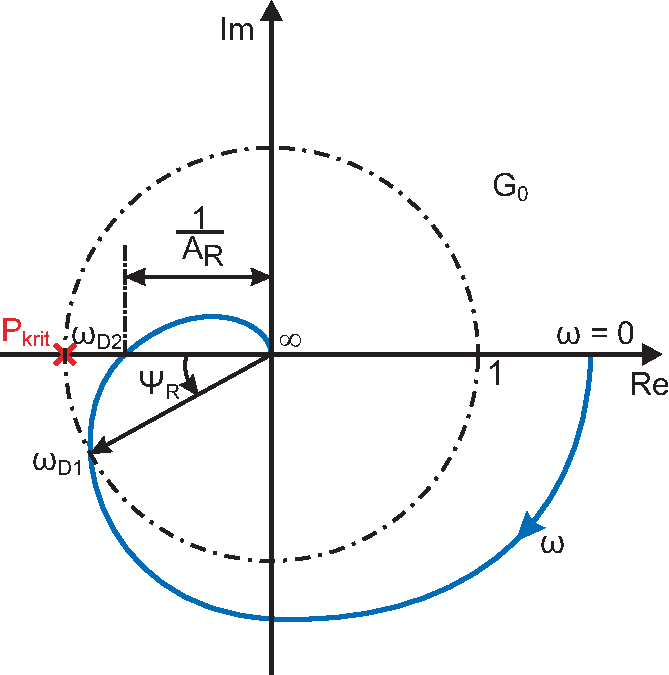
\includegraphics[width=0.6\columnwidth]{Grafiken/Kenngroessen_Ortskurve}
\end{center}

\subsection{Phasenrand- / Amplitudenrandkriterium}
Äquivalent zur Überprüfung der Stabilität des geschlossenen Regelkreises sind das Phasenrand- und das Amplitudenrandkriterium (des offenen Regelkreises). Voraussetzung für die Anwendbarkeit ist, dass $A(\omega_{D1})=1$ nur eine Lösung $\omega_{D1}$ und der offene Kreis keine Pole in der rechten Halbebene hat.
\subsubsection{Phasenrandkriterium}
Der geschlossene Regelkreis ist E/A-stabil, wenn gilt:
\begin{equation*}
\Psi_R>0
\end{equation*}
\subsubsection{Amplitudenrandkriterium}
Der geschlossene Regelkreis ist E/A-stabil, wenn gilt:
\begin{equation*}
A_R>1
\end{equation*}

\section{Reglerentwurf}

\subsection{Heuristische Einstellmethoden}

\subsubsection{Symmetrisches Optimum}
\resizebox{\columnwidth}{!}{
\begin{tabular}{|l|l|l|}
	\hline
	Typ der Regelstrecke & Reglertyp $G_R(s)$ & Reglerparameter\\
	\hline
	\pbox{\columnwidth}{
		\vspace{0.2cm}
		P-Regelstrecke\\\\
		$\frac{K_S}{(1+sT_1)\cdot\prod\limits_{\nu =2}^{n}(1+sT_{\nu})},\;T_1>4\cdot\underbrace{\sum\limits_{\nu=2}^nT_{\nu}}_{T_{\Sigma}}$
		\\\\
	}
	& \multirow{2}{*}{
		\pbox{\columnwidth}{
			PI-Regler\\\\
			$K_I\cdot\frac{1+\tau s}{s}$\\\\
			oder\\
			$K_P+\frac{K_I}{s}, K_P=K_I\cdot\tau$
		}
	}
	& \multirow{2}{*}{
		\pbox{\columnwidth}{
			$\tau=4\cdot\sum\limits_{\nu=2}^nT_{\nu}=4\cdot T_{\Sigma}$\\
			$K_I=\left(2\cdot K_S\cdot \frac{\tau}{T_1}\cdot\sum\limits_{\nu=2}^nT_{\nu}\right)^{-1}$\\
			$=\frac{T_1}{8K_ST_{\Sigma}^2}$
		}
	}\\
	\cline{1-1}
	\pbox{\columnwidth}{
		\vspace{0.2cm}
		I-Regelstrecke\\\\
		$\frac{K_S}{sT_1\cdot\prod\limits_{\nu=2}^n(1+sT_{\nu)}}$
	}
	& & \\
	\hline
		\pbox{\columnwidth}{
			\vspace{0.2cm}
			P-Regelstrecke\\\\
			$\frac{K_S}{(1+sT_1)\cdot (1+sT_2)\cdot\prod\limits_{\nu=3}^n(1+sT_{\nu})},\;T_1>T_2>8\cdot\underbrace{\sum\limits_{\nu=3}^nT_{\nu}}_{T_{\Sigma}}$
			\\\\
		}
		& \multirow{2}{*}{
			\pbox{\columnwidth}{
				PID-Regler\\\\
				$K_I\cdot\frac{(1+s\tau_1)(1+s\tau_2)}{s}$
			}
		}
		& \multirow{2}{*}{
			\pbox{\columnwidth}{
				$\tau_1=\tau_2=8\cdot\sum\limits_{\nu=3}^nT_{\nu}=8\cdot T_{\Sigma}$\\
				$K_I=\left(2\cdot K_S\cdot\frac{\tau_1\cdot\tau_2}{T_1\cdot T_2}\cdot\sum\limits_{\nu=3}^nT_{\nu}\right)^{-1}$\\
				$=\frac{T_1\cdot T_2}{128K_ST_{\Sigma}^3}$
			}
		}\\
		\cline{1-1}
		\pbox{\columnwidth}{
			\vspace{0.2cm}
			I-Regelstrecke\\\\
			$\frac{K_S}{sT_1\cdot(1+sT_2)\cdot\prod\limits_{\nu=3}^n(1+sT_{\nu})},\;T_2>8\cdot\underbrace{\sum\limits_{\nu=3}^nT_{\nu}}_{T_{\Sigma}}$
		}
		& & \\
		\hline
\end{tabular}
}\\\\\\
\textbf{Eigenschaften:}
\begin{enumerate}[label=$\bullet$]
\item Beschleunigtes Einschwingverhalten
\item Gutes stationäres Verhalten
\item Kompromiss zwischen gutem Führungs- und Störverhalten
\item Robustheit gegen Parameteränderungen
\item Überschwingen kann durch einen $PT_1$-Vorfilter leicht kompensiert werden
\end{enumerate}

\subsubsection{Einstellregeln nach Ziegler-Nichols}
\underline{Voraussetzung:}\\
Stabile Strecken mit globalem $P$-Verhalten und S-förmigem Verlauf der Sprungantwort.\\
Die zugrundegelegten Reglertypen sind $P$-, $PI$- oder $PID$-Regler der allgemeinen Form:
\begin{equation*}
G_R(s)=K_R\left(1+T_vs+\frac{1}{T_ns}\right)
\end{equation*}
Zunächst müssen $K_{R,\text{krit}}$ und $T_\text{krit}=\frac{2\pi}{\omega_{\text{krit}}}$ aus der Nyquist-Ortskurve bestimmt werden, die die Schwingbedingung erfüllt:
\begin{equation*}
K_\text{R,krit}\cdot \underbrace{G_S(j\omega_{\text{krit}})}_{\text{Regelstrecke}}\sollsein -1
\end{equation*}
\textbf{Einstell-Regeln:}\\\\
\begin{tabular}{|l|l|l|l|}
\hline
Reglertyp & $K_R$ & $T_n$ & $T_v$\\
\hline
$P$-Regler & $0,5\cdot K_{R,\text{krit}}$ & $(\infty)$ & $(0)$\\
\hline
$PI$-Regler & $0,45\cdot K_{R,\text{krit}}$ & $0,85\cdot T_{\text{krit}}$ & $(0)$\\
\hline
$PID$-Regler & $0,7\cdot K_{R,\text{krit}}$ & $0,4\cdot T_{\text{krit}}$ & $0,15\cdot T_{\text{krit}}$\\
\hline
\end{tabular}

\subsection{Frequenzgangentwurfskriterien}
\begin{center}
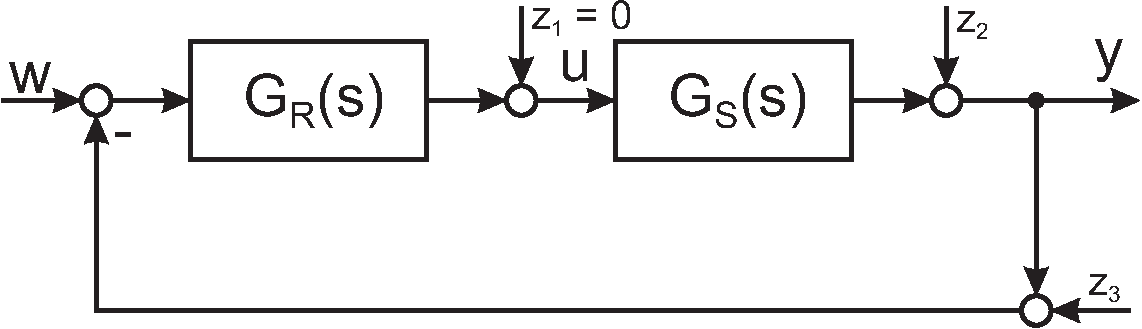
\includegraphics[width=0.8\columnwidth]{Grafiken/Regelkreisentwurf_Grundstruktur}
\end{center}
Für die Regelgröße $y$ gilt:
\begin{equation*}
Y(s)=\underbrace{\frac{G_0(s)}{1+G_0(s)}}_{G_w(s)}W(s)+\underbrace{\frac{1}{1+G_0(s)}}_{G_{z_2}(s)}Z_2(s)+\underbrace{\frac{-G_0}{1+G_0(s)}}_{G_{z_3}(s)}Z_3(s)
\end{equation*}
Für gutes Führungs- und Störungsübertragungsverhalten muss gelten:
\begin{equation*}
G_w\sollseinapprox 1,\;\;\;\;G_{z_2}\sollseinapprox 0,\;\;\;\;G_{z_3}\sollseinapprox 0
\end{equation*}

\subsubsection{Entwurfsvorschriften für zufriedenstellenes Regelkreisverhalten}
\begin{enumerate}
\item Stabiltät:
\begin{equation*}
\Psi_R>0
\end{equation*}
\item Gutes stationäres Verhalten:
\begin{equation*}
\left.|G_0(j\omega)|\right|_{\omega<<\omega_{D1}}>>1
\end{equation*}
\item Gutes Einschwingverhalten:
\begin{enumerate}[label=]
\item Bandbreite: $\omega_B\approx\omega_{D1}$
\item Einschwingzeit: $T_{\text{ein}}\approx\frac{3}{\omega_{D1}}$
\item Geringes Überschwingen:
\begin{enumerate}[label=$\bullet$]
\item $\Psi_R\approx 60^{\circ}\Leftrightarrow$ gutes Folgeverhalten
\item $\Psi_R\approx 30^{\circ}\Leftrightarrow$ gutes Störverhalten
\end{enumerate}
\end{enumerate}
\item Reduktion des Einflusses von Messrauschen $z_3(t)$:
\begin{equation*}
\left.|G_0(j\omega)|\right|_{\omega>>\omega_{D1}}<<1
\end{equation*}
\item Robustheit gegen Modellierungsfehler:\\
$\rightarrow$ meist mit Forderung 4 gut erfüllt
\end{enumerate}

\subsubsection{Praktische Durchführung der Reglerentwurfsaufgabe}
\textbf{Erfahrungswissen:}
\begin{enumerate}[label=$\bullet$]
\item Streckentyp und typische Führungs- und/oder Störsignale bestimmen die Grundstruktur des zu wählenden Reglers
\item $P$-Anteil: Beeinflussung der Bandbreite und somit Einschwingzeit des Regelkreises
\item $I$-Anteil: Beeinflussung der stationären Genauigkeit
\item $D$-Anteil: Beeinflussung des Phasenrandes und damit des Dämpfungsgrades und des Überschwingens
\end{enumerate}

\subsection{Wurzelortskurven (WOK)}
Die WOK beschreibt die ''Wanderung'' der Pole des geschlossenen Regelkreises $G_{RK}$ in Abhängigkeit eines Parameters $g$.\\\\
Sei $G_0(s,g)=\frac{Z_0(s,g)}{N_0(s,g)}$ die Übertragungsfunktion des offenen Regelkreises, dann lautet das charakteristische Polynom des geschlossenen Regelkreises bzw. die Bestimmungsgleichung für die WOK wie folgt (falls Einheitsrückführung):
\begin{equation*}
N_{RK}(s,g)=Z_0(s,g)+N_0(s,g)\sollsein 0
\end{equation*}
Hieraus können die Pole in Abhängigkeit von $g$ berechnet werden.

\subsubsection{Beispiel}
\begin{center}
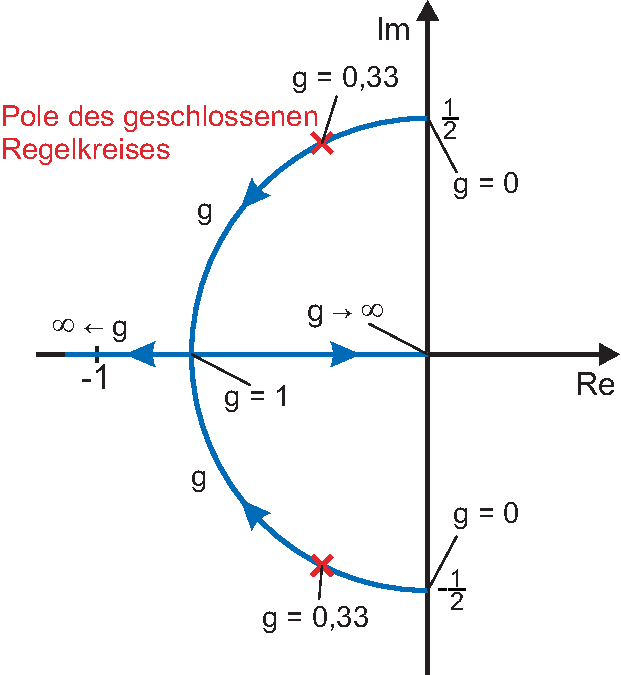
\includegraphics[width=0.8\columnwidth]{Grafiken/WOK_Beispiel}
\end{center}

\subsubsection{Wichtige Eigenschaften}
Falls für die offene Übertragungsfunktion
\begin{equation*}
G_0(s,K)=K\cdot\frac{Z_0(s)}{N_0(s)}=K\cdot Q\frac{\prod\limits_{\mu=1}^{m}(s-q_{\mu}^0)}{\prod\limits_{\nu=1}^{n}(s-p_{\nu}^0)}
\end{equation*}
gilt, wobei $p_{\nu}^0$ und $q_{\mu}^0$ die Pole und Nullstellen des offenen Regelkreises sind und $K$ dem Parameter $g$ entspricht, dann gelten folgende Eigenschaften für die Pole $p_v^{RK}(K)$ des geschlossenen Regelkreises:
\begin{enumerate}[label=$\bullet$]
\item Die Pole $p^{RK}(g)$ liegen stets
\begin{enumerate}[label=-]
\item entweder auf der reellen Achse
\item oder symmetrisch zur reellen Achse
\end{enumerate}
\item $n$ WOK-Äste beginnen für $g=K=0$ in den Polen $p_{\nu}^0$
\item $m$ Äste enden für $K\rightarrow\infty$ in den Nullstellen $q_{\mu}^0$ und die restlichen
\item $n-m$ Äste enden für $g=K\rightarrow\infty$ im Unendlichen. Die Asymptoten dieser Äste schneiden sich im Wurzelschwerpunkt $p_w$:
\begin{equation*}
p_w=\frac{\sum\limits_{\nu=1}^{n}p_{\nu}^0-\sum\limits_{\mu=1}^{m}q_{\mu}^0}{n-m}
\end{equation*}
\item Die Asymptoten schließen mit der reellen Achse einen Winkel
\begin{equation*}
\begin{split}
\Phi_l&=\frac{(2l-1)\pi}{n-m}\;\;\;\;\text{für }KQ>0\\
\Phi_l&=\frac{(2l-2)\pi}{n-m}\;\;\;\;\text{für }KQ<0
\end{split}
\end{equation*}
ein, wobei $l=1,...,(n-m)$
\item $KQ>0$/($KQ<0$): Ein Punkt der reellen Achse ist genau dann Teil der Wurzelortskurve des geschlossenen Kreises, wenn die Anzahl der rechts von dem Punkt liegenden Pole und Nullstellen des offenen Kreises ungerade (gerade oder null) ist.
\end{enumerate}

\section{Strukturelle Erweiterungen der einschleifigen Regelungsstruktur}

\subsection{Führungsgrößenaufschaltung/Vorsteuerung}
\begin{center}
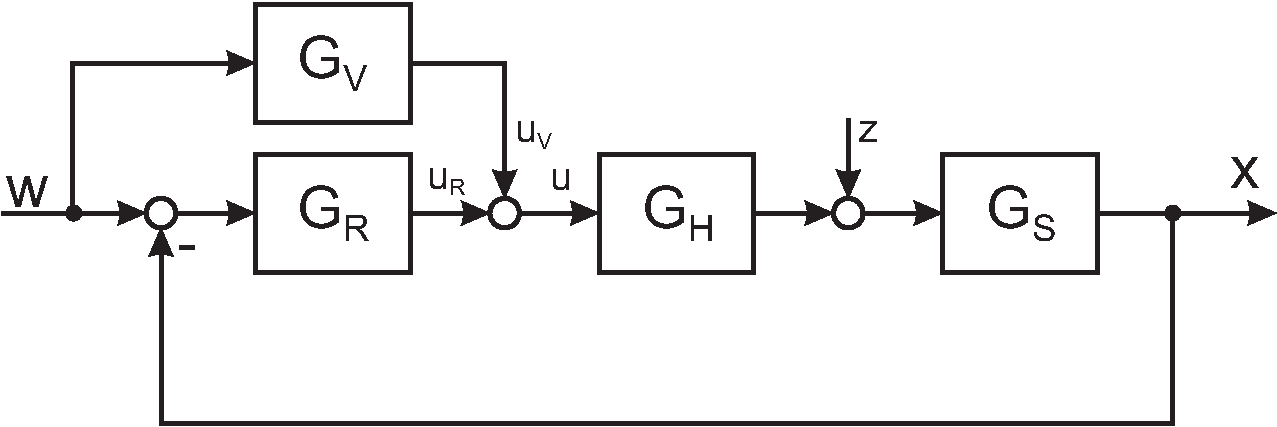
\includegraphics[width=0.95\columnwidth]{Grafiken/Vorsteuerung_Regelkreis}
\end{center}
Wähle
\begin{equation*}
\begin{split}
G_V(s)&=\frac{1}{G_H(s)G_S(s)}\\
\Rightarrow G_w(s)&=\frac{X(s)}{W(s)}=1
\end{split}
\end{equation*}
Da dies allerdings i.d.R. nicht kausal und somit nicht realisierbar ist, wählt man meist als grobe Näherung eine statische Vorsteuerung mit
\begin{equation*}
G_{V,\text{stat}}(s)=\frac{1}{G_H(0)G_S(0)}=\frac{1}{K_HK_S}
\end{equation*}

\subsection{Störgrößenaufschaltung}
\begin{center}
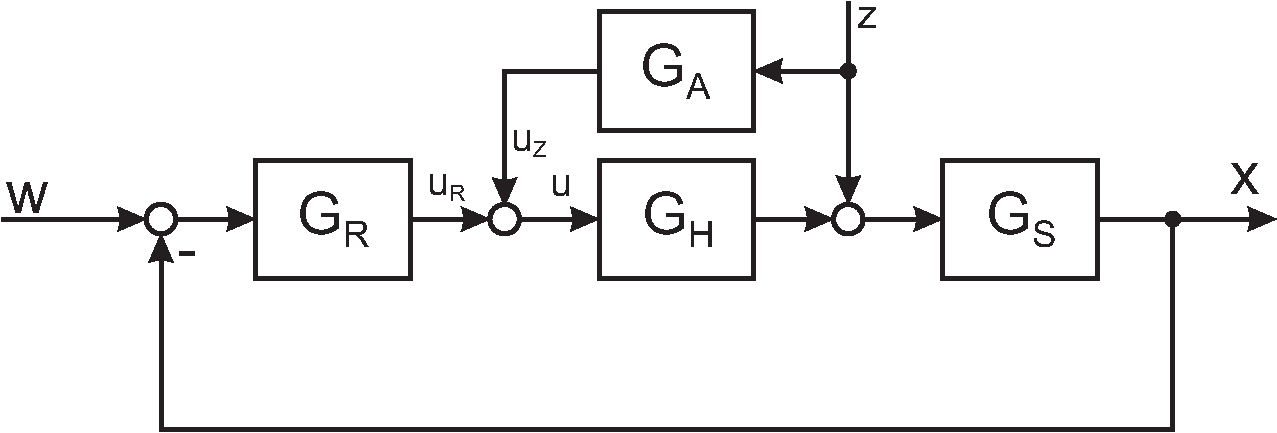
\includegraphics[width=0.95\columnwidth]{Grafiken/Stoergroessenaufschaltung_Regelkreis}
\end{center}
Wähle
\begin{equation*}
\begin{split}
G_A(s)&=-\frac{1}{G_H(s)}\\
\Rightarrow G_z(s)&=\frac{X(s)}{Z(s)}=0
\end{split}
\end{equation*}
Da $G_A(s)$ i.d.R. nicht kausal ist, kann das Störverhalten nur stationär, aber nicht dynamisch verbessert werden:
\begin{equation*}
G_{A,\text{stat}}(s)=-\frac{1}{G_H(0)}=-\frac{1}{K_H}
\end{equation*}

\subsection{Kaskadenregelung}
Kaskadenregelungen sind ineinander verschachtelte Regelkreise, deren dynamisches Verhalten von außen nach innen zumeist schneller wird.
\begin{center}
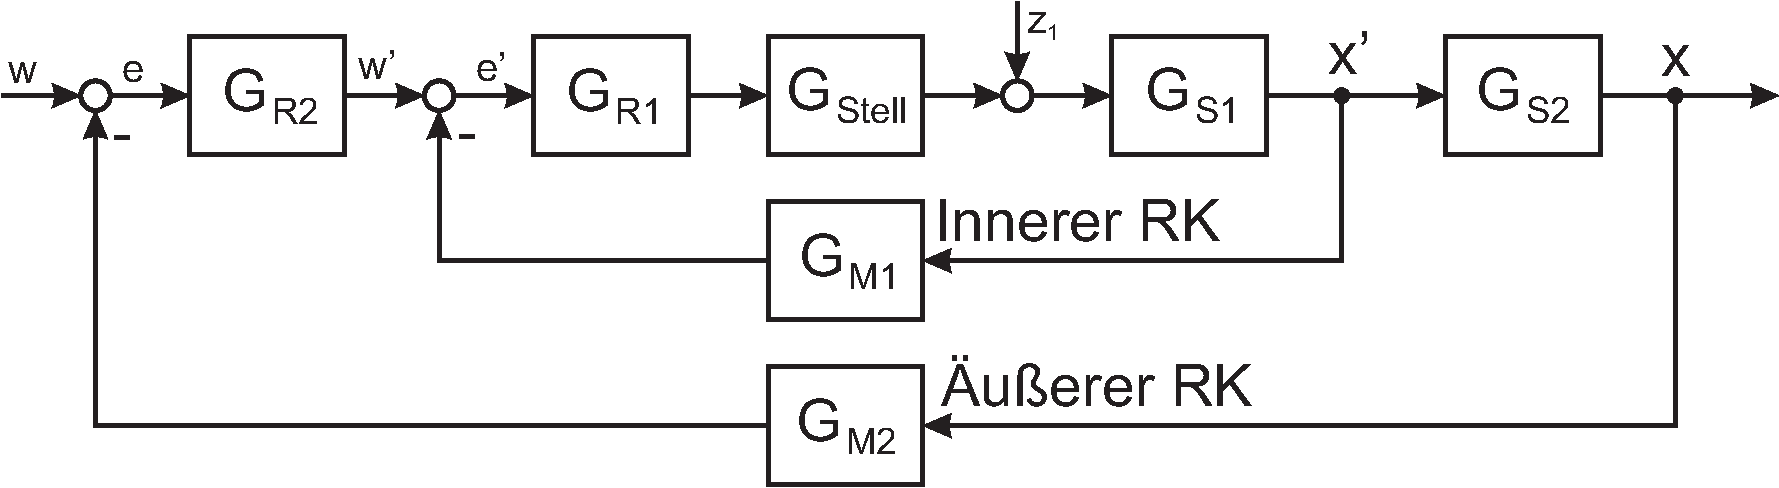
\includegraphics[width=0.95\columnwidth]{Grafiken/Kaskadenregelung}
\end{center}
Falls der innere Regelkreis deutlich schneller als der äußere reagiert, so gilt aus der Sicht des äußeren:
\begin{equation*}
G_w'(s)=\frac{X'(s)}{W'(s)}\approx 1
\end{equation*}

\section{Zustandsbasierter Reglerentwurf}

\subsection{Zustandsregelung von LTI-SISO-Systemen}

\subsubsection{$P$-Regler mit vollständiger linearer Zustandsrückführung}
Das Regelgesetz lautet:
\begin{equation*}
u=K_R\left(w'-\underline{k}^T\underline{x}\right)
\end{equation*}
Mit $\underline{\dot{x}}=A\underline{x}+\underline{b}u,y=\underline{c}^T\underline{x}$ folgt dann:
\begin{equation*}
\underline{\dot{x}}=\underbrace{\left(A-\underline{b}\underline{k}^TK_R\right)}_{A_{\text{Reg}}}\underline{x}+\underline{b}K_Rw'
\end{equation*}
\textbf{Eigenwert- oder Polverschiebungssatz:}\\
Die $n$ Eigenwerte $\lambda_i(A)$ einer vollständig steuerbaren SISO-Strecke $(A,\underline{b})$ können mittels vollständiger linearer Zustandsregelung mit $\underline{k}\in\mathbb{R}^n$ zu beliebigen Regelungseigenwerten verschoben werden.

\subsubsection{Reglerentwurf durch Polverschiebung oder -zuweisung}
\begin{enumerate}
\item Ist $(A,\underline{b})$ vollständig steuerbar?\\
Wenn ja, dann nach 2); sonst ist keine vollst. EW-Verschiebung möglich
\item Wahl der Regelungspole $p_{\nu}$ mit gewünschten dynamischen Eigenschaften:
\begin{equation*}
N_{\text{Reg}}^{\text{soll}}(s)=\prod\limits_{\nu=1}^n(s-p_{\nu})
\end{equation*}
\item Ist-Nennerpolynom bestimmen:
\begin{equation*}
N_{\text{Reg}}^{\text{ist}}(s,\underline{k})=det\left(sI_n-A_{\text{Reg}}(\underline{k})\right)\;\;\text{mit }A_{\text{Reg}}=A-\underline{b}\underline{k}^T
\end{equation*}
\item $\underline{k}$ durch Koeffizientenvergleich bestimmen:
\begin{equation*}
N_{\text{Reg}}^{\text{soll}}=N_{\text{Reg}}^{\text{ist}}
\end{equation*}
\end{enumerate}

\subsection{Zustandsbeobachter}
Ein Zustandsbeobachter schätzt $\underline{\hat{x}}$, falls $\underline{x}$ nicht vollständig direkt messbar ist.

\subsubsection{Parallelmethode}
$x_1(t)$ kann entweder aus $u(t)$ oder aus $y(t)$ bestimmt werden:
\begin{center}
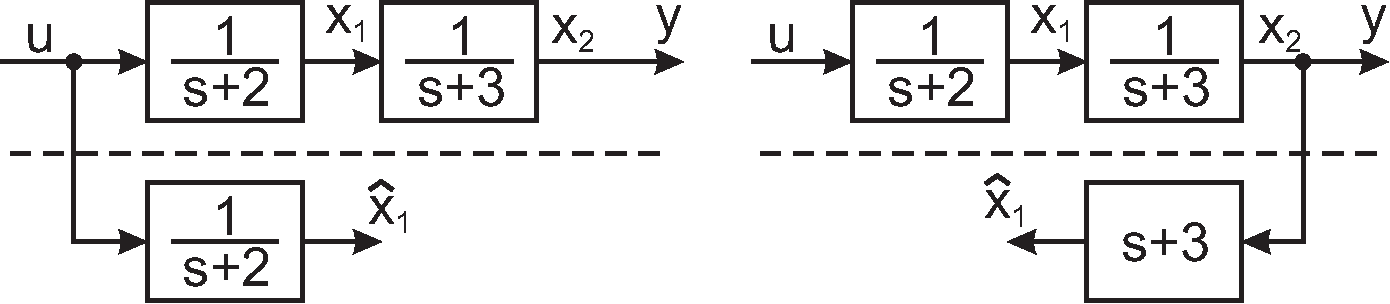
\includegraphics[width=0.95\columnwidth]{Grafiken/Parallelmodellmethode}
\end{center}
Die linke Methode ist hierbei weniger empfindlich gegenüber Messrauschen.\\
Deshalb wird die rechte Methode nur dann eingesetzt, wenn $u$ nicht messbar oder das linke Teilsystem instabil ist.

\subsubsection{Vollständiger Zustandsbeobachter}
\begin{equation*}
\begin{split}
\underline{\dot{\hat{x}}}&=\underbrace{(A-\underline{l}\underline{c}^T)}_{\hat{A}=A_{\text{Beo}}}\underline{\hat{x}}+\underline{b}u+\underline{l}y=\underbrace{A\underline{\hat{x}}+\underline{b}u}_{\text{Prozessmodell}}+\underbrace{\underline{l}(y-\hat{y})}_{\text{Korrekturterm}}\\
\hat{y}&=\underline{c}^T\underline{\hat{x}}\\
u&=K_vw-\underline{k}^T\underline{\hat{x}}
\end{split}
\end{equation*}
\textbf{Beispiel:}
\begin{center}
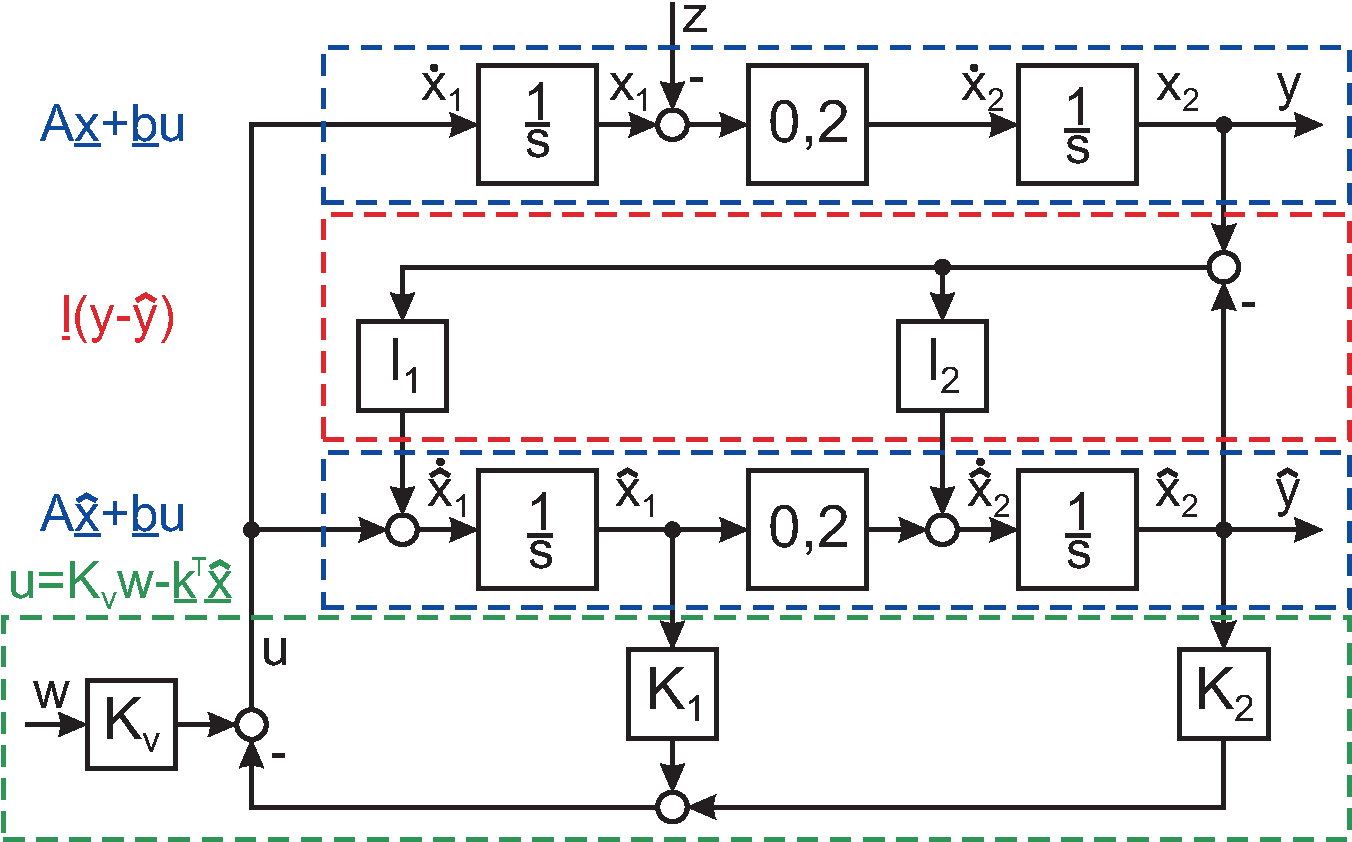
\includegraphics[width=0.95\columnwidth]{Grafiken/Vollst_Zustandsbeobachter}
\end{center}
\textbf{Eigenwert- oder Polverschiebungssatz für Beobachter:}\\
Die $n$ Eigenwerte $\lambda_i(A)$ eines vollständig beobachtbaren Prozessmodells $(A,\underline{c}^T)$ können mit Hilfe des Beobachter-Rückführverktors $\underline{l}\in\mathbb{R}^n$ zu beliebigen Beobachtereigenwerten verschoben werden.\\\\
\underline{Faustregel zur Bestimmung von $\underline{l}$:}
\begin{equation*}
Re\{\lambda_i(\hat{A})\}\leq Re\{\lambda_i(A)\}\;\;\forall i
\end{equation*}
\underline{Schätzfehler:}
\begin{equation*}
\underline{\tilde{x}}=\underline{\hat{x}}-\underline{x}\rightarrow \underline{\dot{\tilde{x}}}=\hat{A}\underline{\tilde{x}}-\underline{g}v
\end{equation*}

\subsection{Zustandsregelung unter Einschluss eines Beobachters}
\begin{center}
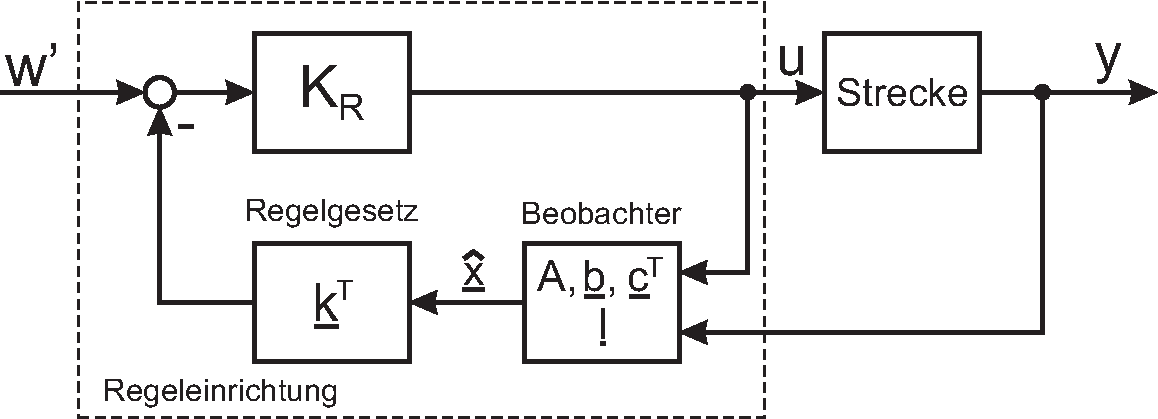
\includegraphics[width=0.95\columnwidth]{Grafiken/Zustandsregler_mit_Beobachter}
\end{center}

\subsubsection{Dynamischer Zustandsraum-Kompensator}
= aus Zustandsregler und -beobachter zusammengesetzte Regeleinrichtung.
\begin{center}
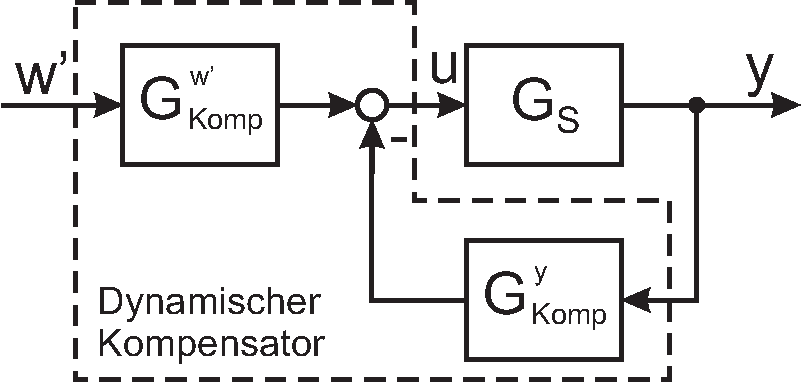
\includegraphics[width=0.6\columnwidth]{Grafiken/Zustandsraum-Kompensator}
\end{center}
\begin{equation*}
\begin{split}
G_{\text{Komp}}^{w'}(s)&=-\underline{k}^T(sI_n-A_{\text{Komp}})^{-1}\underline{b}+1\\
G_{\text{Komp}}^y(s)&=-\underline{k}^T(sI_n-A_{\text{Komp}})^{-1}\underline{l}=-\frac{det\begin{bmatrix}(sI_n-A_{\text{Komp}}) & -\underline{l} \\ \underline{k}^T & 0\end{bmatrix}}{det[sI_n-A_{\text{Komp}}]}
\end{split}
\end{equation*}
mit $A_{\text{Komp}}=A-\underline{l}\underline{c}^T-\underline{b}\underline{k}^T$

\section{Zeitdiskrete Realisierung zeitkontinuierlicher Regelungsgesetze und Modelle}

\subsection{Zustandsdarstellungen}
\begin{equation*}
\begin{split}
\underline{x}_{k+1}&=A\underline{x}_k+\underline{b}u_k\\
\underline{y}_k&=\underline{c}^T\underline{x}_k+\underline{d}u_k
\end{split}
\end{equation*}
Erweiterte Standardform:
\begin{equation*}
\underline{x}_{k+1}=A\underline{x}_k+\underline{b}u_k+\underline{b}_1u_{k+1}\\
\end{equation*}

\subsection{Differenzengleichung $n$-ter Ordnung}
\begin{equation*}
a_ny_{k-n}+a_{n-1}y_{k-n+1}+...+a_0y_k=b_mu_{k-m}+...+b_0u_k
\end{equation*}

\subsection{$\mathcal{Z}$-Übertragungsfunktion}
\begin{equation*}
X(z)=\mathcal{Z}\{x(t)\}=\sum\limits_{k=0}^{\infty}x(k)z^{-k}
\end{equation*}

\subsubsection{Wichtige Eigenschaften}
\begin{enumerate}[label=$\bullet$]
\item Linearität:
\begin{equation*}
\mathcal{Z}\{x_k+y_k\}=X(z)+Y(z)
\end{equation*}
\item Differenzensatz:
\begin{equation*}
\mathcal{Z}\{x_{k+n}\}=z^nX(z)-z^nx_0-z^{n-1}x_1-...-zx_{n-1}
\end{equation*}
\end{enumerate}

\subsection{Zeitverhalten und Analyse zeitdiskreter LTI-Systeme}

\subsubsection{Allgemeine Lösungsformel zur Zustandsform}
\begin{equation*}
\underline{x}_k=A^k\underline{x}_0+\sum\limits_{j=0}^{k-1}A^{k-j-1}\underline{b}u_j,\;\;\;k=1,2,3,...
\end{equation*}

\subsubsection{Stabilität}
System ist asymptotisch stabil, falls
\begin{equation*}
|\lambda_i(A)|<1,\;\;i=1,2,...,n
\end{equation*}
$\Rightarrow$ Stabilitätsgebiet ist Einheitskreisscheibe\\\\
\textbf{Achtung:}\\
Zur Berechnung der Eigenwerte muss $G(z)$ gegebenenfalls so erweitert werden, dass die niedrigste Potenz von $z$ gleich $0$ ist ($z^0=1$).

\subsection{Methoden der Zeitdiskretisierung von LTI-Systemen}
\begin{tabular}{ll}
$\underline{\dot{x}}=\tilde{A}\underline{x}+\tilde{B}\underline{u}$ & $\Rightarrow \underline{x}_{k+1}=A\underline{x}_k+B\underline{u}_k+B_1\underline{u}_{k+1}$\\
$y=\tilde{C}\underline{x}+\tilde{D}\underline{u}$ & $\Rightarrow \underline{y}_k=C\underline{x}_k+D\underline{u}_k$
\end{tabular}\\\\
mit $\underline{x}_k=\underline{x}(t_k)=\underline{x}(kh)$.

\subsubsection{Rechteck-Approximation}
Hierbei wird die Integration durch ein Rechteck angenähert.
\begin{equation*}
\Rightarrow s\entspr\frac{1-z^{-1}}{h}
\end{equation*}
\begin{equation*}
\begin{split}
A&=[I_n-\tilde{A}h]^{-1}\\
B&=0,\;B_1=[I_n-\tilde{A}h]^{-1}h\tilde{B}\\
C&=\tilde{C},\;\;D=\tilde{D}
\end{split}
\end{equation*}

\subsubsection{Trapez-Approximation}
Hierbei wird die Integration durch ein Trapez angenähert.
\begin{equation*}
\Rightarrow s\entspr\frac{2(z-1)}{h(z+1)}
\end{equation*}
\begin{equation*}
\begin{split}
A&=\left[I_n-\tilde{A}\frac{h}{2}\right]^{-1}\left[I_n+\tilde{A}\frac{h}{2}\right]\\
B&=B_1=\left[I_n-\tilde{A}\frac{h}{2}\right]^{-1}\frac{h}{2}\tilde{B}\\
C&=\tilde{C},\;\;D=\tilde{D}
\end{split}
\end{equation*}

\subsubsection{Sprunginvarianzmethode}
Hierbei wird die Eingangsgröße $\underline{u}(t)$ durch eine Stufenfunktion $\underline{u}(t_k)$ approximiert.\\\\
\textbf{Berechnung im Zeitbereich:}
\begin{equation*}
\begin{split}
A&=e^{\tilde{A}h}\\
B&=\int\limits_0^he^{\tilde{A}\eta}d\eta\tilde{B}=\left(e^{\tilde{A}h}-I_n\right)\tilde{A}^{-1}\tilde{B}\\
C&=\tilde{C},\;\;D=\tilde{D}
\end{split}
\end{equation*}
\textbf{Berechnung im Frequenzbereich:}
\begin{equation*}
G(z)=\left(1-z^{-1}\right)\mathcal{Z}\left[\frac{G(s)}{s}\right]
\end{equation*}

\subsection{Rekursiver Simulationsalgorithmus}
Gegeben sei:
\begin{equation*}
G(z)=\frac{Y(z)}{W(z)}=\frac{b_0+b_1z^{-1}+...+b_mz^{-m}}{a_0+a_1z^{-1}+...+a_nz^{-n}}
\end{equation*}
Transformiere wie folgt:
\begin{equation*}
\begin{split}
z^{-i}Y(z)&\Laplace y_{k-i}\;\;\forall i\\
z^{-i}W(z)&\Laplace w_{k-i}\;\;\forall i
\end{split}
\end{equation*}
und löse anschließend nach $y_k$ auf.

\subsection{Festlegung der Abtastfrequenz $f_A$ in Regelkreisen}

\subsubsection{Ermittlung von $T_A$ anhand der Sprungantwort}
Es gelten folgende Faustformeln:
\begin{equation*}
\begin{split}
\omega_A&\approx 20\omega_g\\
15\omega_B&\leq\omega_A\leq 50\omega_B\\
\omega_A&=\frac{2\pi}{T_A}
\end{split}
\end{equation*}
\textbf{Vorgehensweise zum Ermitteln von $T_A$ aus $G(s)$:}
\begin{enumerate}
\item Berechnen der Impulsantwort:
\begin{equation*}
G(s)\Laplace g(t)
\end{equation*}
\item Berechnen der Sprungantwort:
\begin{equation*}
h(t)=\int\limits_0^tg(\tau)d\tau
\end{equation*}
\item
\begin{equation*}
T'=\frac{h(t\rightarrow\infty)}{g(t=0)}
\end{equation*}
\item Siehe Diagramm:
\end{enumerate}
\begin{center}
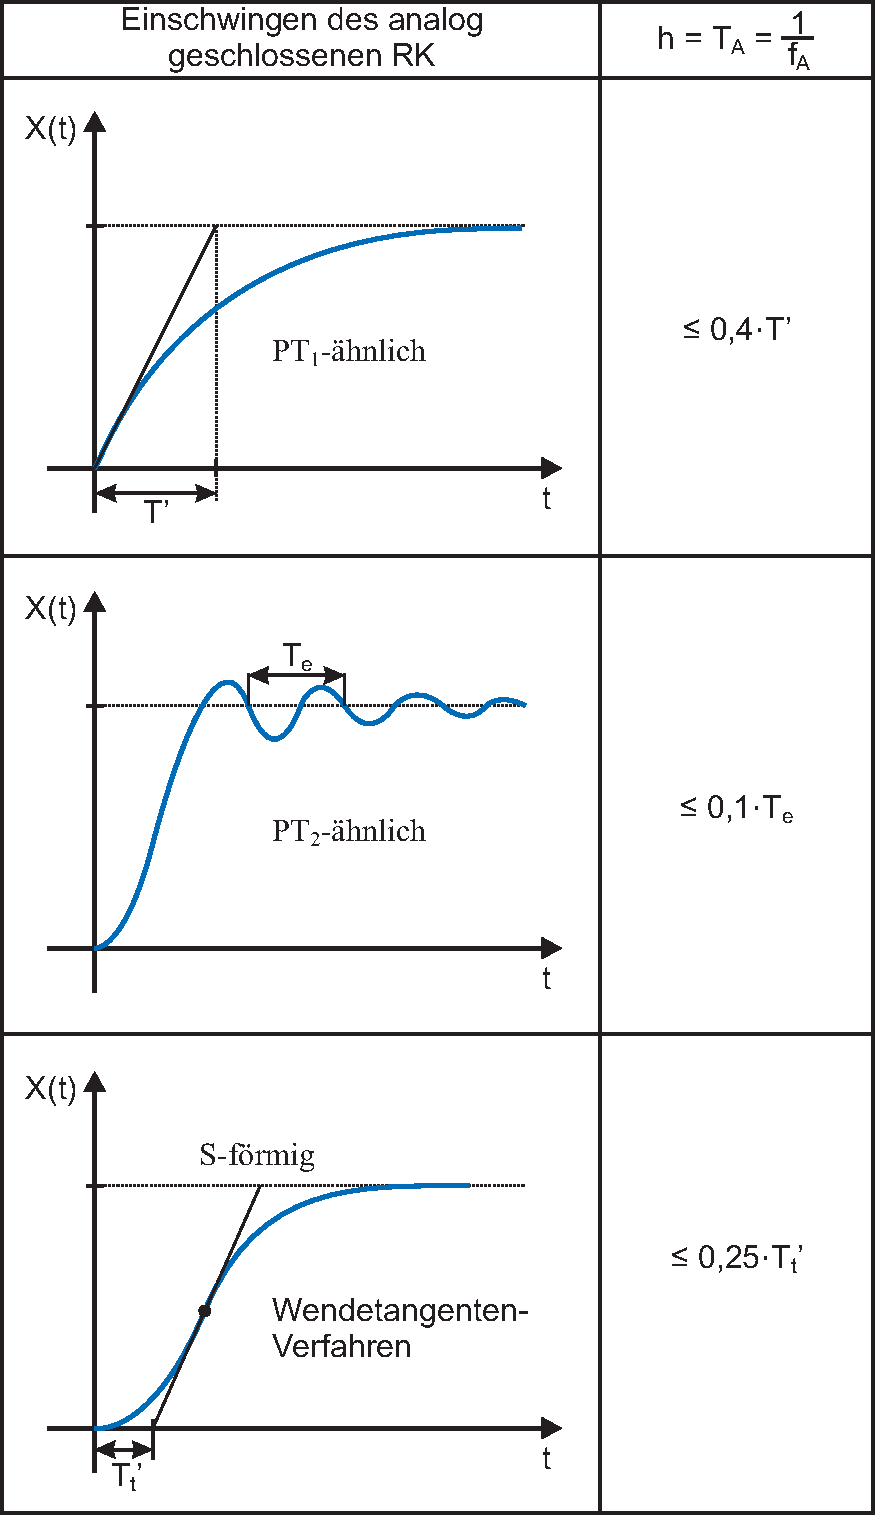
\includegraphics[width=0.85\columnwidth]{Grafiken/Faustformeln_Einschwingverhalten}
\end{center}

\subsubsection{Schutzfilter}
Durch die Filterung des Sensorsignales vor seiner Abtastung kann die Rückfaltung des Messrauschens deutlich reduziert werden.
\begin{enumerate}[label=$\bullet$]
\item Butterworth-Filter 1. Ordnung $\rightarrow$ einfach
\begin{equation*}
G_r(s)=\frac{0,5\omega_A}{s+0,5\omega_A}
\end{equation*}
\item Butterworth-Filter 2. Ordnung $\rightarrow$ steilere Flanke
\begin{equation*}
G_r(s)=\frac{(0,5\omega_A)^2}{s^2+\sqrt{2}(0,5\omega_A)s+(0,5\omega_A)^2}
\end{equation*}
\end{enumerate}
Zur Berechnung des minimales Dämpfungsfaktors der Messstörungen muss $|G_r(j\omega_{UG})|$ berechnet werden\\
($\omega_{UG}$: untere Grenzfrequenz des Messrauschens). 
\\\\\\\\
Lizenz: CC BY-NC-SA 3.0\\
\url{http://creativecommons.org/licenses/by-nc-sa/3.0/de/}

\end{document}








